\documentclass[sigconf, review=true, screen=true, anonymous=true]{acmart}

\usepackage{booktabs}
\usepackage[ruled]{algorithm2e} % For algorithms

\usepackage{siunitx}
\usepackage{graphicx}
\usepackage{caption}
\usepackage{subcaption}
\usepackage{multirow}
\usepackage{todonotes}
\usepackage[capitalise]{cleveref}

\renewcommand{\algorithmcfname}{ALGORITHM}
\SetAlFnt{\small}
\SetAlCapFnt{\small}
\SetAlCapNameFnt{\small}
\SetAlCapHSkip{0pt}
\IncMargin{-\parindent}

% Metadata Information
%\acmConference{SAP}
%\acmVolume{9}
%\acmNumber{4}
%\acmArticle{39}
%\acmYear{2010}
%\acmMonth{3}
%\acmArticleSeq{11}

%Copyright
\setcopyright{usgovmixed}

% DOI
\acmDOI{0000001.0000001}

% Paper history
\received{March 2018}

\begin{document}

\title{An Audio Interface for an Active Perception Navigation Aid for Blind People}

\author{Jacobus C. Lock}
\affiliation{%
  \institution{University of Lincoln}
  \streetaddress{Brayford Pool}
  \city{Lincoln}
  \state{Lincolnshire}
  \postcode{LN6 7TS}
  \country{United Kingdom}}

\author{Iain Gilchrist}
\affiliation{%
  \institution{University of Bristol}
  \streetaddress{Priory Road}
  \city{Bristol}
  \state{Bristol}
  \postcode{BS8 1TU}
  \country{United Kingdom}}

\author{Grzegorz Cielniak}
\affiliation{%
  \institution{University of Lincoln}
  \streetaddress{Brayford Pool}
  \city{Lincoln}
  \state{Lincolnshire}
  \postcode{LN6 7TS}
  \country{United Kingdom}}

\author{Nicola Bellotto}
\affiliation{%
  \institution{University of Lincoln}
  \streetaddress{Brayford Pool}
  \city{Lincoln}
  \state{Lincolnshire}
  \postcode{LN6 7TS}
  \country{United Kingdom}}

\begin{abstract}
	Our aim is to build a portable active navigation system for the visually impaired that uses active perception techniques and a combination of feedback modes to identify a scene and guide a user to their destination.
	Such a system requires a non-visual feedback interface and in this paper we investigate the effectiveness of a spatial audio tone with a varying pitch component, played through bone-conducting headphones, in conveying the pan and tilt angles of a target to the user in a pointing task.
	The goal is to determine how changes to the rate of change of the pitch affects a user's performance.
	For this, wee conducted a set of experiments with blindfolded and visually impaired users and found that the varying pitch component gives an average error of approximately \SI{20}{\degree} when searching for a target; in line with previous results from other authors.
	Furthermore, we are able to demonstrate that the audio interface adheres to Fitts's Law and used it as a metric to determine which pitch setting produces the optimal results.
	We discovered a trade-off between the speed and accuracy in the pointing task, which are maximised when the tone's pitch is adjusted to a low and high rate of change respectively. 
\end{abstract}

 \begin{CCSXML}
<ccs2012>
<concept>
<concept_id>10003120.10003121.10011748</concept_id>
<concept_desc>Human-centered computing~Empirical studies in HCI</concept_desc>
<concept_significance>500</concept_significance>
</concept>
<concept>
<concept_id>10003120.10003121.10003122.10003334</concept_id>
<concept_desc>Human-centered computing~User studies</concept_desc>
<concept_significance>300</concept_significance>
</concept>
</ccs2012>
\end{CCSXML}

\ccsdesc[500]{Human-centered computing~Empirical studies in HCI}
\ccsdesc[300]{Human-centered computing~User studies}

\keywords{Human-machine interface, vision impairment, navigation aid, spatialised sound, Fitts's Law, pointing task}

\maketitle
\renewcommand{\shortauthors}{JC Lock et al.}

\section{Introduction}

In recent years, governments have spearheaded numerous initiatives to support people with disabilities and enable them to play a more active role in modern society.
In the UK, the Royal National Institute of Blind People (RNIB) has prioritised enabling people with visual impairments to use some of the services and products many people take for granted, such as public transport and cellphones~\cite{rnib-objectives}.
Improvements in modern computing have made it possible for new and innovative solutions for these problems to come to the fore.
In particular, researchers in the field of active vision have have made much progress in enabling machines to autonomously manipulate cameras to gain more information about an environment to complete mapping and object and face tracking tasks, for example~\cite{bajcsy2018revisiting}.
There is, however, a significant research question about whether techniques from active machine vision can be applied to humans, i.e.\ can a machine identify a point of interest in a scene and direct a human, instead of an electronic servo, to focus a camera on that point?
If this can be done, it would be beneficial to people with visual impairments and will augment their ability to search for an arbitrary point of interest or identify an unknown scene. 

To this end, we are developing a mobile device-based navigation system using a Google Project Tango device\footnote{https://developers.google.com/tango}, pictured in \cref{fig:tango-headphone}, that caters to the perception limitations of people with limited vision by using a non-visual interface.
This system will ultimately allow users with visual impairments to reach a target location in the final leg of their journey, i.e.\ the so-called `last 10 yards' problem~\cite{google2016blind,bellotto2013}. 
The ideas here can also be extended and applied to mainstream navigation tools, such as Google Maps.
A Tango-enabled device comes pre-equipped with powerful image-processing, localisation and depth-perception capabilities and is built on top of a standard Android platform, providing access to the entire set of input/output options that this operating system has to offer.
The final system will use multiple feedback modes (vibration, audio and voice) to guide a user toward a target destination while providing information on any oncoming obstacles.

%\begin{figure}
  %\centering
  %\begin{subfigure}[t]{0.45\textwidth}
\begin{figure}
  \centering
  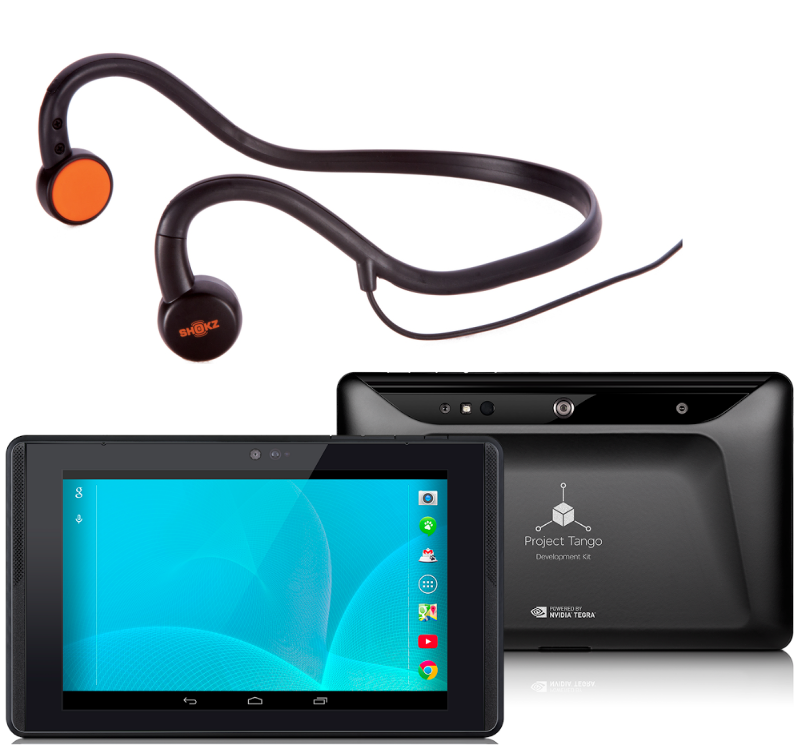
\includegraphics[width=0.4\textwidth]{figures/tango_headphone.png}
  \caption{The Tango device and bone-conducting headset used by the participants. }\label{fig:tango-headphone}
\end{figure}
  %\end{subfigure}\hfill
  %\begin{subfigure}[t]{0.45\textwidth}
  %\end{subfigure}
  %\caption{The hardware used during the experiment, as well as a diagram showing the Tango device's coordinate system. }
%\end{figure}

In this paper we focus on the audio feedback mode and discuss how it is used in our system.
We present experiments we performed to determine its effectiveness at directing a user to complete a pointing task and how its parameters affect users' target-search performance.
For the pointing task, we presented blindfolded and partially sighted participants with a set of virtual targets, one after another, and asked them to point a camera to where they thought the targets were.
The targets' pan and tilt angles ($\phi$ and $\theta$ respectively) w.r.t.\ the Tango's vertical plane, shown in \cref{fig:cam-coords}, were given to the participants through a spatial tone with varying pitch played via a set of bone-conducting headphones.
We use the latter to not interfere with the user's normal hearing function, which people with visual impairments typically rely on.
Because these headphones bypass the external structure of the ear responsible for localising a sound source's elevation, it is necessary to convey the target's tilt angle using another method.
Therefore, we opted for a tone with varying pitch to convey the angle adjustment required to point the camera in a particular direction.

\begin{figure}
  \centering
  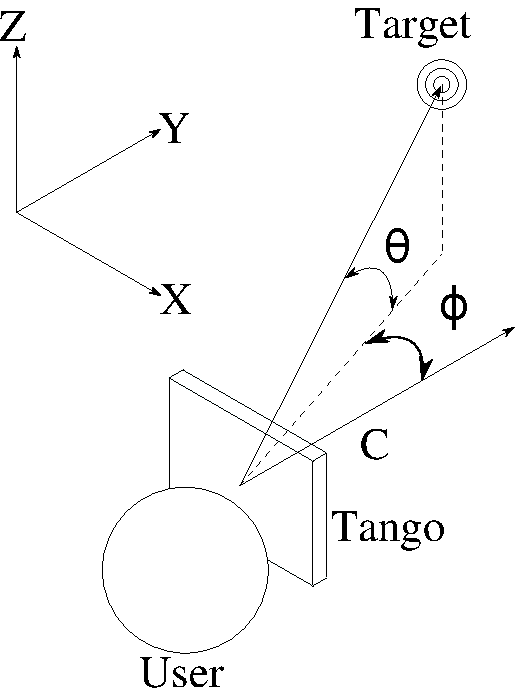
\includegraphics[width=0.4\textwidth]{figures/camera_coordinate.pdf}
  \caption{A diagram showing the Tango's frame of reference and the target's pan ($\phi$) and tilt ($\theta$) angles.}\label{fig:cam-coords}
\end{figure}

Unfortunately, there is a gap in the literature regarding the use of a such an audio interface for pointing tasks with regards to a mobile device.
It is also unclear whether popular metrics, such as Fitts's Law~\cite{fitts1954information}, can be applied in this case.
Fitts's Law is a predictive model in the field of psychomotor research, often used in the human-machine interfacing field, that relates the time it takes a user to direct a pointing device toward a target as a function of the difficulty of finding the target (i.e.\ the ratio between the distance to the target and its size).
If a Fitts relationship is found, it can be used as a metric to anticipate whether future adjustments to the pitch's rate of change will have a positive effect on target-search performance.

The main contributions of this paper are two-fold: 

\begin{itemize}
  \item we provide the first experimental results on how well a tone with varying pitch can convey a target's tilt angle when using a mobile device with bone-conducting headsets; 
  \item we show that this sound-based human-machine interface conforms to Fitts's Law and can provide a useful metric of performance for similar mobile user interfaces.
\end{itemize}

The remainder of this paper is organised as follows: \cref{sec:lit-review} gives an overview of existing navigation systems and audio interfaces for people living with visual impairments.
\cref{sec:portable-navigation} discusses the navigation device's hardware and interface setup and describes how $\phi$ and $\theta$ are conveyed to the user.
The experiments that were conducted are explained in \cref{sec:experiments} and the results are presented and discussed in \cref{sec:results}. 
Finally, \cref{sec:conclusion} concludes this paper with a summary of the findings and comments on our future work. 

\section{Previous Work}\label{sec:lit-review}

\todo{chop up this section. Make anonymous}
Attempting to deliver a system that allows people with visual impairments to independently navigate and accomplish everyday tasks is not new; in fact, there are multiple commercial systems and research prototypes already available on the market.
One approach that has been investigated is to outfit the existing white walking cane with various sensors,
such as sonar, radar, motor encoders, etc.~\cite{ulrich1997, marion2008batcane} to warn the user of upcoming obstacles, instead of relying on haptic feedback from the impact between the cane and the obstacle.
Another approach is to outfit a walking cane to act as a radio-frequency identification (RFID) antenna that can read a set of RFID tags placed at strategic locations around the environment at key spots or along a path~\cite{faria2010electronic, willis2005}.
This modification to the traditional cane is more discreet than the systems mentioned earlier and has been shown to work well.
Bluetooth tags and a smartphone can also be used in a similar manner~\cite{sato2017navcog3}.
However, the major drawbacks here are the significant cost and effort of modifying existing infrastructure with RFID and Bluetooth tags and maintaining them to stay up to date with a changing environment.
GPS-based systems~\cite{ran2004drishti, loomis2001navigating, kammoun2012navigation}, while cheap and reliable in outdoor environments, are not applicable in built-up urban areas and indoors where GPS signals are notoriously unreliable.
Computer vision-based systems provide a good compromise between usability, cost and accuracy and have been the focus of much research recently~\cite{manduchi2014last}.
One increasingly popular solution is to use RGB-D depth sensing cameras, which are becoming increasingly more accurate and cost-effective, to build a 3D image map of the environment, allowing a user to safely traverse through it~\cite{lee2015, rodriguez2012obstacle}.
Another approach is to use vision-based object recognition techniques to detect various objects and landmarks, such as doors, staircases, etc., and communicate their relative location to the user~\cite{schauerte2012assistive, tian2013b, fiannaca2014headlock}, or use audio instructions to instruct a user with vision impairment to fully capture an object of interest~\cite{vazquez2012helping}. 

An important feature of user-centric systems is a human-machine interface (HMI) that enables effective and seamless two-way communication between the system and the user.
In previous surveys, researchers found that people with visual impairments prefer receiving feedback and instructions in the form of speech and haptic feedback cues~\cite{khoo2016multimodal, ross2000wearable, vazquez2012helping}.
However, haptic feedback modes typically have a lower bandwidth when compared to audio feedback and also require the user to wear a special device in order to transmit the haptic signals to the user effectively.
Work has also been done in translating a visual scene into non-visual formats, with so-called sensory substitution systems (e.g. `The Voice'~\cite{meijer2010}) and virtual audio reality (VAR) systems~\cite{frauenberger2003} reporting favourable results.
However, The Voice, while helpful, has a very steep learning curve that has proven to be a significant barrier to entry.
With VAR systems, it is not clear how unknown environments, where markers have not yet been encoded, would be handled and described to the user. 

Spatial audio has also been considered to convey the direction of a target.
Experiments have previously determined that people are able to find the location of a stationary sound source with an error of $\pm$\SI{35}{\degree}, in both the pan and tilt dimensions~\cite{zwiers2001spatial}, for both early-blind and normally-sighted people.
However, in~\cite{lewald2013exceptional, lessard1998early} it was found that the blind have a clear advantage in localisation accuracy over sighted people when presented with more difficult tasks, such as targets in motion and narrow-band stimuli, with~\cite{lewald2013exceptional} reporting an average absolute localisation error of around \SI{10}{\degree} in the pan and tilt dimensions.
Other authors found that the minimum difference in the spatial sound's angle for the user to be able to perceive movement is approximately \SI{1.7}{\degree}. During the experiments, an audio speaker was physically manoeuvred to provide the participant with a spatialised sound tone~\cite{ashmead1998spatial}.
Researchers have also tried using simulated spatial audio to inform the user from which direction a sound is originating~\cite{holland2002audiogps, kammoun2012navigation, rebillat2009smart, menelas2010audio, wilson2007swan, zotkin2004rendering}.
In these works, a sound was played through a set of headphones and the source spatialised with a head-related transfer function (HRTF), tricking the listener into thinking the sound source was located at some arbitrary 3D location.
Various audition techniques and methods were then used to guide the user along a path.
Other authors have also provided a framework for evaluating the quality of this 3D sound in terms of its psychoacoustic properties~\cite{guastavino2004perceptual, nicol2014roadmap}.
There are also experimental results about how well users can find targets presented with spatial sound in the tilt and panning dimensions with normal headphones~\cite{katz2011spatial, zwiers2001spatial}, as well as work that has shown similar levels of localisation performance between normal and bone-conducting headphones in the pan dimension~\cite{macdonald2006spatial}.
However, to our knowledge no extensive work or experiments have been done to determine how well users respond to tilt adjustment instructions using a tone with \emph{varying pitch}, in particular when using bone-conducting headphones. 

Researchers have previously used Fitts's Law~\cite{fitts1954information}, and more recently MacKenzie's modified version of it~\cite{mackenzie1992fitts}, as a metric to evaluate the performance of a spatial audio HMI\@.
Fitts's Law was originally proposed for visual target search tasks.
However, it has been applied in non-visual target search tasks as well.
For example, experiments with a haptic feedback pointing device have been performed to evaluate how effective it was at directing a user towards a target~\cite{ahmaniemi2009augmented}.
The authors showed that the search time adheres to Fitts's Law.
However, they also note that it is not a perfect fit, citing the fact that Fitts's Law does not take into account a user's search strategy.
Another group of researchers conducted experiments using a spatial audio interface to describe the position of a target on the horizontal plane~\cite{marentakis2006effects}.
Here, participants pointed to where they thought the targets were, on their left or right, as they traversed a path.
Their results show a good relation between target difficulty and search time, providing a strong argument that Fitts's Law can be used to describe the performance of a spatial audio interface.
These results have since been supported by other authors, who found that Fitts's Law provided a good explanation for the results from an experiment using visual, limited visual and non-visual feedback cues~\cite{wu2010fitts}.
However, Fitts's Law has not yet been shown to apply to a spatial tone that uses varying pitch to convey the target's tilt angle, as demonstrated in this paper.

\section{Portable Navigation System}\label{sec:portable-navigation}

\subsection{System Setup}

We intend to ultimately deliver a portable navigation device that is capable of guiding a user with visual impairments on the last leg of their journey, e.g.\ to a specific aisle and shelf in a shop.
To do this, we will use a combination of different feedback modes to facilitate two-way communication between the user and the device.
A large amount of data need to be translated from a visual form into a format that is useful to people with limited or no vision.
We therefore plan to use a combination of voice, audio and vibration cues to translate visual navigation data as effectively as possible and overcome the bandwidth limitation of the human ear. 

%The system is based on a concept proposed in~\cite{bellotto2013, lock2017portable}, which uses a Google Tango device.
This is an Android-based cellphone or tablet device that comes equipped with an RGB-D camera to sense colour and depth.
It combines an inertial measurement unit with powerful and robust landmark recognition and image processing algorithms to localise itself in real-time.
An added benefit of this platform is its familiar, compact form-factor which will help overcome the hurdle of user-acceptance and usability.

We use a set of bone-conducting headphones (see \cref{fig:tango-headphone}) that are placed externally on a user's head so that the system does not occlude the perception of real-world sounds and does not interfere with a user's normal hearing function.
In the future, we will use multiple feedback modes to provide the user with navigation and obstacle avoidance instructions.
However, for this paper, we only considered the spatialised audio mode and its variation in pitch in order to determine its effectiveness in conveying a target's pan and tilt angles.

A diagram of the experimental system pipeline is shown in \cref{fig:pipeline}.
Here, the arrows indicate the direction of the flow of information.
When the user taps the Tango's screen, a new virtual target is generated and its coordinates are sent to the audio generation module, along with the Tango's current position and orientation.
The audio generator then produces a tone based on the difference between the Tango and the target's positions (in the Tango's global coordinate system) and sends it to the audio output channel, which plays it back to the user.
The WiFi recording module is constantly monitoring the different parameter values of the Tango and target's positions, as well as the system's output, and records it to a remotely stored datafile. 

\begin{figure}
  \centering
  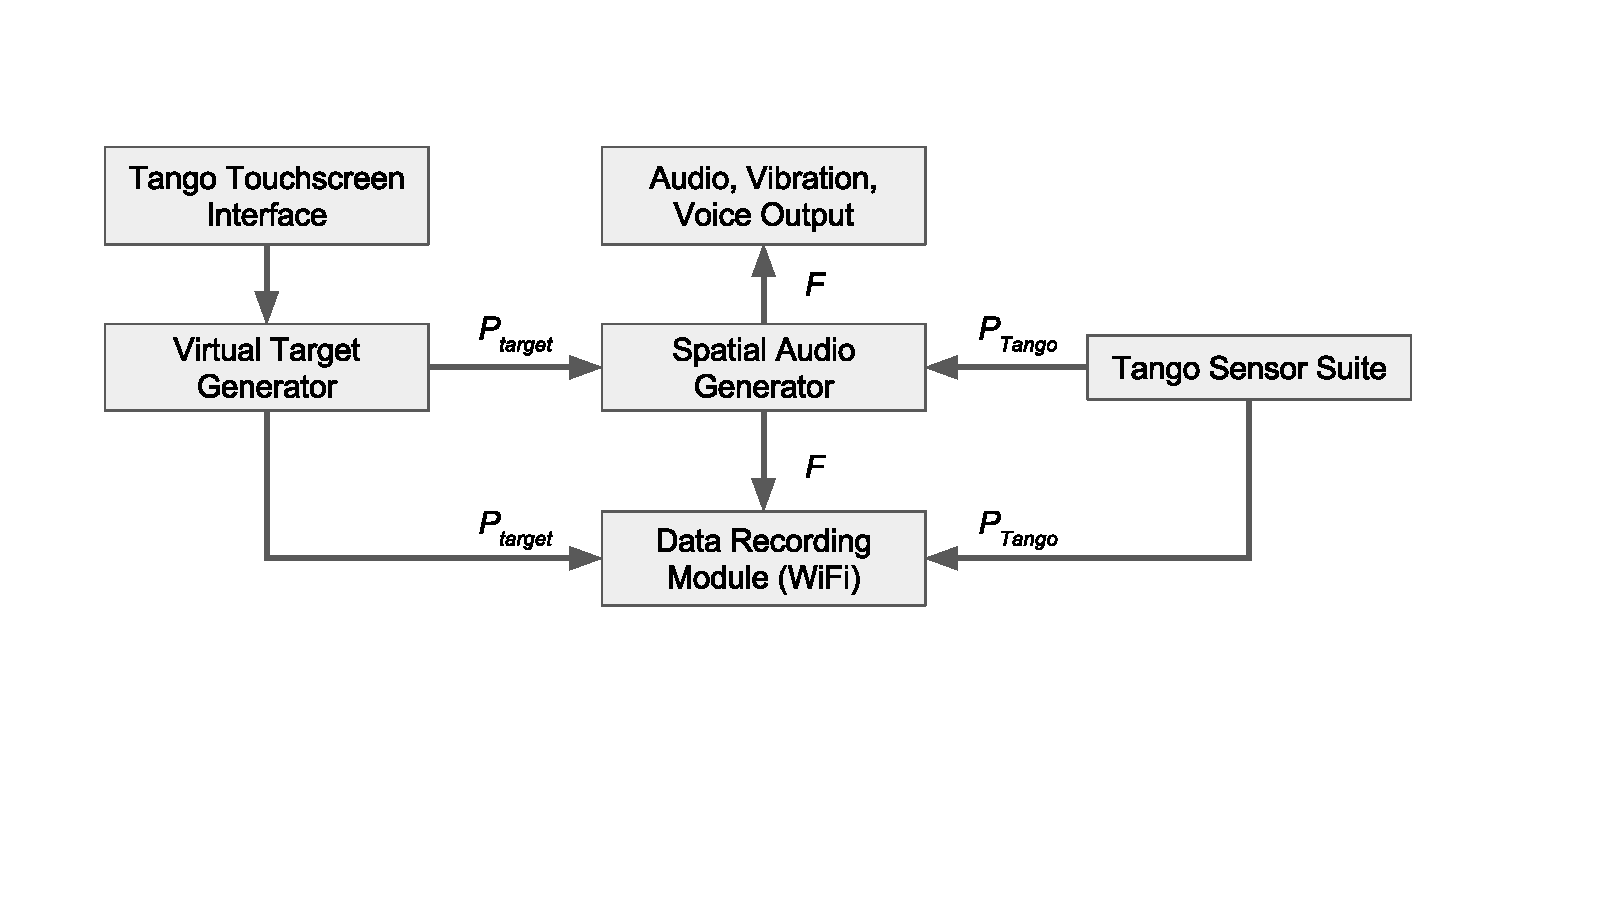
\includegraphics[clip=true, trim=50 120 80 50, width=0.4\textwidth]{figures/pipeline.pdf}
  \caption{A diagram of the individual system components and their communication pipelines. $F$ indicates a feedback signal and $P$ a pose signal. }\label{fig:pipeline}
\end{figure}

\subsection{Audio Interface}

For the series of experiments performed in this work, only the audio feedback mode was used to interface with the user.
The audio component is responsible for conveying the 2D position of a target on the vertical plane w.r.t.\ the Tango's coordinate system, showed in \cref{fig:cam-coords}, in terms of pan and tilt angles.
In future system iterations, the distance to a target can be rendered by adjusting the audio signal's amplitude as a function of the distance.
The audio signal is a continuous $\sim$\SI{10}{\hertz} sinusoidal sound wave that is played to the user through bone-conducting headphones.
We select a sinusoidal wave because it is relatively simple to manipulate and analyse.
A richer and more natural tone will be implemented at a later stage of the project. 

The audio is spatialised in the pan dimension using the OpenAL\footnote{http://openal.org} sound library's HRTF, while the tilt angle is conveyed by varying the audio tone's pitch.
We use this approach because the external set of bone-conducting headphones plays the sound through a user's cheekbones instead of their outer ears, bypassing the ears' pennae that provide humans their ability to localise elevated sound sources~\cite{roffler1968factors, algazi2001elevation}.
This makes an HRTF less effective in conveying the target's tilt angle and therefore needs to be conveyed using another method; a varying pitch tone in this case.
The difference between the target's angular position and the device's angular orientation are used to generate the audio signals. 

\subsubsection{Pan Direction}

The pan angle ($\phi$) describes the angle which the user needs to rotate the camera vector around the $z$-axis in \cref{fig:cam-coords}, i.e.\ how far the target is to the left or right of the user.
We use an HRTF to add a spatial element to the audio tone that is played to the user, making the tone sound like it is coming from the direction of the target.
Humans determine a sound source's pan direction by subconsciously analysing the time difference between a sound reaching both of your ears.
For example, if you hear a sound in your left ear first, you interpret the sound as coming from your left.
The greater the so-called inter-aural time difference, the greater the perceived angular distance to the sound source~\cite{wightman1992dominant}.

We implement OpenAL's default HRTF, based on the MIT's KEMAR dataset\footnote{sound.media.mit.edu/resources/KEMAR.html}, to generate a sinusoidal sound wave based on the difference between the user and target's positions.
The library takes position values as input and outputs a tone based on the angle between the two position vectors. 

\subsubsection{Tilt Direction}

The system adjusts the tone's pitch ($f$) to convey the target's tilt angle ($\theta$) w.r.t.\ the camera's current pointing vector, $C$, as shown in \cref{fig:cam-coords}. 
Here, a high pitch means the target is above the camera vector (i.e.\ the user should look up) and a low pitch means the target is below the camera vector (the user should look down).
This high/low association scheme is chosen because humans naturally associate high-pitched sounds with higher objects and lower-pitched noises with lower objects~\cite{pratt1930spatial, blauert1997spatial}.
We use a logarithmic, octave-based gain function for the pitch, since an increase in octave provides a distinct perceptible change while keeping the timbre roughly constant~\cite{shepard1964circularity}.

We wish to determine how the gradient of the pitch gain as a function of $\theta$ (i.e.\ $m = \frac{df}{d\theta}$) affects a user's performance.
For example, does steeper $\frac{df}{d\theta}$ lead to an increased target acquisition rate?
For this we select three different pitch settings, referred to henceforth as $m_l$, $m_m$ and $m_h$ for the smallest, middle and highest gain gradients respectively. 
To find these gradients, we set the maximum and minimum limits for $\theta$ and the maximum and minimum frequencies for $f$.
Furthermore, for the sake of consistency, each gradient setting is set to generate the same pitch when the user is pointing the camera towards the target. 

After practical tests with the Tango and headphones, we set the neutral, on-target tone to $f_{512} =$ \SI{512}{\hertz} for its audibility.
For $m_l$, we set $f_{max}$ and $f_{min}$ to one octave higher and lower than the neutral tone, giving limits of \SI{1024}{\hertz} and \SI{256}{\hertz} respectively.
For $m_m$, the $f_{max}$ and $f_{min}$ are set to two octaves higher and lower than the neutral tone (\SI{2048}{\hertz} and \SI{128}{\hertz}) and $m_h$ to three octaves higher and lower (\SI{4096}{\hertz} and \SI{64}{\hertz}).
We selected these limits for practical reasons, given the fact that the bone conducting headphones we use have low volume gain at very high and low frequencies, making it difficult to hear. 
The values of $m_l, m_m, m_h$ are visualised in \cref{fig:pitch-gain}.
$f$ is given by \cref{eq:pitch-eq}, where $c$ can be found using the current pitch setting's pitch and angle limits.

\begin{equation}\label{eq:pitch-eq}
  f = 2^{-m \theta + c}
\end{equation}

\begin{figure}
  \centering
  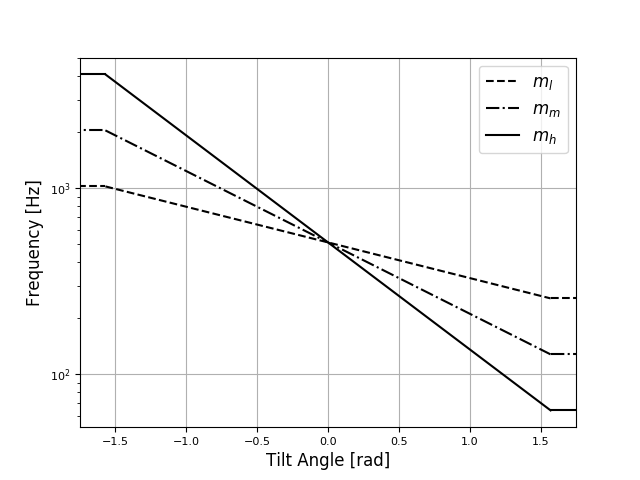
\includegraphics[width=0.4\textwidth]{figures/pitch_gain_functions.png}
  \caption{The pitch gain functions for the 3 different gain settings. }\label{fig:pitch-gain}
\end{figure}

The \SI{0}{\radian} position is directly in front of the user.
We set the range of angles the system can convey to $[-\frac{\pi}{2}; \frac{\pi}{2}]$; anything outside this range implies that the target is behind the user and was not considered in this series of experiments. 

\section{Experiments}\label{sec:experiments}

We performed a set of experiments with our audio interface to determine its effectiveness at directing a user to adjust a camera's $\phi$ and $\theta$ to point it to a target.
%Furthermore, we also carried out a set of pre-screening experiments to determine each participant's hearing characteristics.
The results from the experiments allow us to better understand how the users respond to different settings for the spatial audio feedback stimulus and use them to improve and optimise the behaviour of the feedback modes in our portable navigation aid.

The participants were given time before the experiments commenced to familiarise themselves with the device and the tones it emits, as well as what the $f_{512}$ `on-target' tone sounds like.
We also tested the system with 3 legally blind participants and compared their data to the blindfolded dataset.
These tests in particular provided us with subjective feedback on the system that can be used to improve future iterations.

\subsection{Experimental Procedure}

For the experiments we used two groups of participants, with one including 42 sighted and blindfolded participants and the other 3 legally blind volunteers with varying degrees of vision impairment. 
They performed a series of experiments using our system with a pair of bone-conducting headphones.
The participants were recruited on a volunteer-basis and consisted of a diverse group of undergraduate students and professionals with ages ranging between 17 and 40 years (13 male, 32 female) and did not not have significant hearing issues or any other disability that could affect the experiment.

%The participants participated in three experiments.
%The first two experiments were performed to determine each participant's hearing characteristics and provide some context to the results generated during the target-search experiment.
%These characterisation experiments will also indicate pre-existing biases our participant-base might have in the modes or dimensions we performed our third experiment on: the target search. 

%\begin{figure}
  %\centering
  %\begin{subfigure}[t]{0.45\textwidth}
    %\centering
    %\includegraphics[width=0.5\textwidth]{figures/sighted_participant.png}
    %\caption{A sighted and blindfolded participant. }
  %\end{subfigure}\hfill
  %\begin{subfigure}[t]{0.45\textwidth}
    %\centering
    %\includegraphics[width=0.5\textwidth]{figures/vi_participant2.jpg}
    %\caption{A visually impaired participant. }
  %\end{subfigure}
  %\caption{Participants in the study using the Tango device during the target-search task. }
  %\label{fig:participants}
%\end{figure}

We are only evaluating the interface in the pan and tilt dimensions and the 3D targets are therefore generated at a constant distance of \SI{2}{\metre} from the participant.
Throughout the experiments, various parameters of the target and the participant are recorded and streamed in real-time to a laptop computer via a WiFi connection.
Prior to the target search experiment, the blindfolded participant group was given a few minutes without a blindfold to familiarise themselves with the system and confirm the target's location with their own eyes.
This was done verbally with the participants with limited vision. 

%\subsection{Participant Characterisation}

%\subsubsection{Spatial Awareness}

%In this experiment, we evaluated a participant's ability to determine the lateral direction a sound is coming from.
%To do this, we played a continuous \SI{512}{\hertz} sinusoidal tone to the participant through the headphones and applied an HRTF to spatialise and place its source to the participant's left or right.
%The participant then had to select the direction the sound came from.
%The longer the experiment lasts and the more correct guesses the participant makes, the closer the source moves to the centre-front of the participant, making it increasingly difficult to localise. 

%For this progressive increase in difficulty, a 2-up, 1-down step process is used~\cite{wetherill1965sequential,levitt1971transformed}, meaning that for every 2 correct answers, the distance to the centre halves, making the lateral direction harder to determine.
%Conversely, the task becomes easier for each incorrect answer by doubling the sound source's distance from the centre.
%We also use 2 different step sequences, one starting at a large distance (\SI{45}{\degree}) from the user and the other at the minimum distance (approximately \SI{1}{\degree}), giving an `easy' and a `hard' step respectively.
%The terminating condition for the experiment is when the 2 step sequences converge to within 2 step ranges of one another for 3 consecutive guesses.
%This gives a distance band within which the participant is capable of localising the sound source. Each participant performed this experiment three times. 

%\subsubsection{Pitch Discrimination}

%Here we determined a participant's ability to differentiate pitch, i.e.\ how well they can tell if a tone is high or low pitched.
%We played 2 tones to the participants in succession with the second tone being higher or lower-pitched than the first.
%The participants were then asked to select whether they interpreted the second tone as higher or lower-pitched than the first.

%The first tone is randomly generated, while the second tone is generated by adding or subtracting some value from the first one.
%The tone difference depends on how well the participant can tell the tones apart.
%Like the spatial awareness experiment, a 2-up, 1-down step process is used: for every 2 consecutive correct answers, the pitch difference between the tones is halved, and the difference is doubled for every incorrect answer.
%Two step sequences are again used here, one starting with a large pitch difference ($f_h=2^9=$ \SI{512}{\hertz}) between the tones and the other with a small difference ($f_l=2^1=$ \SI{2}{\hertz}).
%The termination condition is when the two step sequences are within one octave of each other (i.e.\ $\log_2\frac{f_h}{f_l}=2^1$) for 3 consecutive answers.
%Each participant performed this experiment twice. 

%\subsection{Target Search}

\subsection{Task Description}

The final experiment is the main one and will answer the question we are most interested in: how well does a spatial tone with varying pitch direct a user to look in a specific direction and how do the parameters of this tone affect the user's performance in this task? 

For this experiment, the participants were blindfolded where necessary and given a Tango device running an app purpose-written for this experiment.
When started, a set of virtual targets were presented one at a time to the participant on the Tango device.
Then, depending on the direction the participant was currently pointing the camera relative to the target's position, the Tango generated and played a tone via the bone-conducting headphones to indicate the pan and tilt angle adjustment required to point the camera to the target. %These instructions are spatialised tones with varying pitch: an HRTF indicates the pan direction (left or right) and the pitch indicates whether the participant should be looking up (high pitch) or down (low pitch) to find the target. 

Once the participant pointed the camera toward the target, the system generated a neutral tone with a pitch of \SI{512}{\hertz}, which we used as the `on-target' pitch for all of our experiments.
The participants then had to manually confirm the direction they believe the target was after hearing the on-target tone and tap the screen.
At this point a new search target was presented and the search-process was repeated.
To minimise any speed/accuracy trade-off bias in the results, we asked the participants to search for the targets without placing particular emphasis on accuracy or time. 

28 targets were presented to each participant per run.
The positions of these targets were randomly generated and equally spread across the 4 quadrants on the vertical plane to prevent a clustering of targets at the same location.
After every run of the experiment, the parameters controlling the tone's behaviour was adjusted.
In this case, the rate of change of the tone's pitch was adjusted to make the pitch increase at a lower or higher rate as a function of the tilt angle between the target and the participant's current pointing direction.
This was done to see whether, for example, a more rapid increase in pitch would help the participant find the target faster or more accurately.
The order in which the settings were set for each participant was randomised in order to minimise any learning effect the participant population might display between each experiment. 

\subsection{Metrics}

We use two different metrics to compare the three different pitch gradient settings: the acquisition accuracy and search time.
The accuracy is given as the difference between the Tango's orientation at the time the participant confirmed they were on target, and the target's actual orientation.
We separate the results of the tilt and pan dimensions in order to see how the different pitch gradients affect a participant's pointing accuracy. 

We also compare the performance of the three pitch gradient settings in terms of the time it takes each participant to find a target.
However, since each participant was presented with a different, randomly generated set of targets, a direct time comparison is not possible.
Instead, we use Fitts's Law~\cite{fitts1954information}, modified by MacKenzie for uncertain target sizes and noisy data~\cite{mackenzie1992fitts}, which states that there is a relation between the time it takes to find a target and its index of difficulty (the ratio between the distance to the target and its width).
It also provides a so-called `index of performance' that we can use as a metric to compare the results between the three configurations. 

Here we briefly summarise the equations and quantities involved in our metric.
Fitts's Law is given by  

\begin{equation}
  \label{eq:fitts-base}
  t = a + bID,
\end{equation}

\noindent
where $t$ is the time it takes to find a target, $a$ and $b$ are constants determined through regression and $ID$ is a description of the difficulty of the target, given as logarithmic function of the ratio between the distance to the target and the target's width.
In our case, the targets have no width, since they are points in space, and we therefore use MacKenzie's modified form for $ID$, given by

\begin{equation}
  \label{eq:fitts-id}
  ID = \log_2\left(\frac{\theta}{w_e} + 1\right).
\end{equation}

\noindent
Here $\theta$ is the angular distance between subsequent target centres and $w_e$ is the targets' effective angular width~\cite{welford1968fundamentals}, given by

\begin{equation}
  \label{eq:fitts-we}
  w_e = \sqrt{2\pi e}\sigma = 4.133\sigma,
\end{equation}

\noindent
where $\sigma$ is the standard deviation of the error data, taken as the angle between the participant's target selection and target's actual angular position.
Fitts's index of performance, $IP$, can then be calculated using 

\begin{equation}
  \label{eq:fitts-performance}
  IP = \frac{ID}{t},
\end{equation}

\noindent
where $IP = \frac{1}{t}$ when $\sigma=0$.

\section{Experiment Results and Discussion}
\label{sec:results}

%\subsection{Participant Characterisation}
%\label{sec:character}

%\cref{fig:location-guesses} shows the results for the spatial awareness experiment in the pan direction where the participants had to determine the location of the sound they were played. 

%\begin{figure}
  %\centering
  %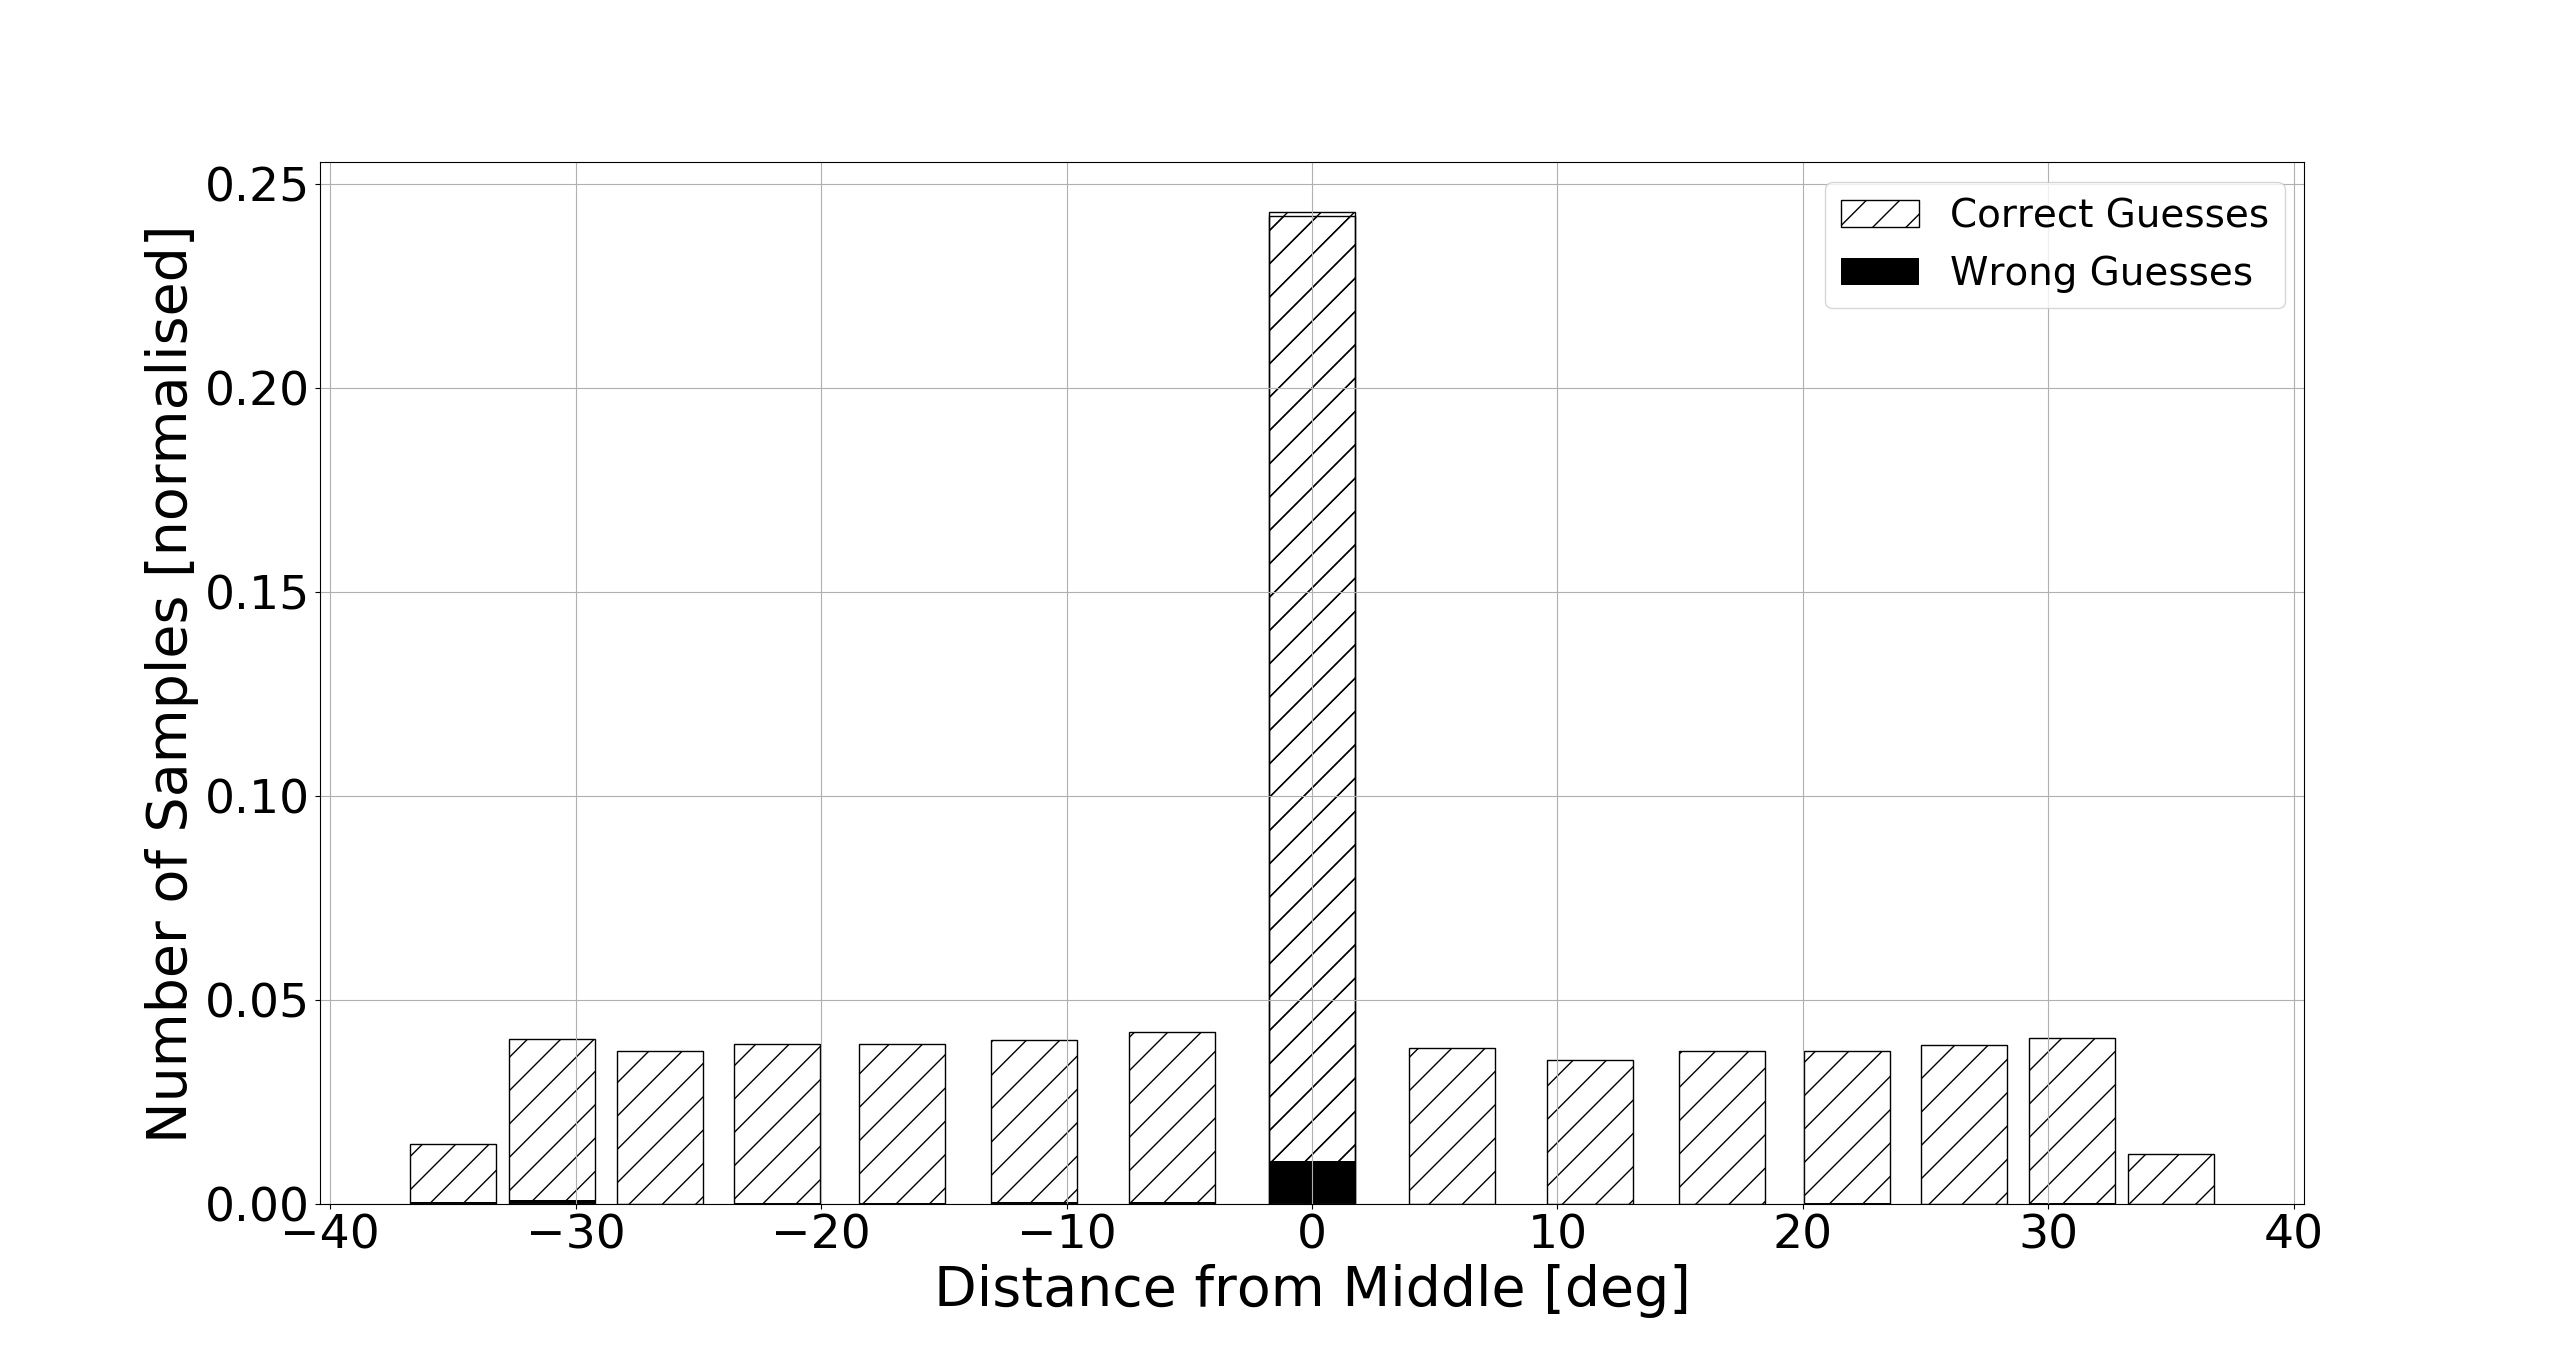
\includegraphics[clip, trim=100 20 150 100, width=0.4\textwidth]{figures/location_guesses.png}
  %\caption{Histograms of the spatial awareness experiment in the pan dimension showing the proportion of correct/incorrect guesses per bin interval. }
  %\label{fig:location-guesses}
%\end{figure}

%With the relatively low number of erroneous guesses, we see that the participants were accurate in guessing the location of the sound source.
%This is further supported by the large number of samples at the minimum difference of \textasciitilde\SI{3}{\cm}, indicating that the participants reached this level more frequently and consistently.
%We can therefore conclude that the participants had little difficulty determining the pan angle of a sound source.
%These results are in line with what we expected and they are supported by literature which indicates that humans are very adept at localising a sound source, and this ability was apparent for the HRTF-generated pan locations. 

%The results recorded during the pitch discrimination experiment are shown in \cref{fig:tone-guesses}, where a bar plot is used to show the number of correct guesses for each tone difference level.
%The latter is given in terms of the relative semitone difference between the tones which are obtained using the following relation: 

%\begin{equation}
%\label{eq:semitone-difference}
  %\Delta f = 12\log_2\frac{f_0}{f_1}.
%\end{equation}

%From \cref{fig:tone-guesses}, we can see that the guesses are normally spread around a 0 semitone difference.
%As expected, a larger proportion of incorrect guesses occur around the smaller differences with the majority of samples for correct and incorrect guesses being recorded in the $[-0.25, 0.25]$ semitone difference level.
%Assuming these differences are normally distributed, we fitted a cumulative distribution function (CDF) over each participant's set of results for their correct guesses and used the CDF's parameters to determine the semitone difference threshold, where the participant could no longer reliably tell two tones apart, for each participant.
%See \cref{fig:cdf-semitone} for an example showing the actual CDF of a participant and its approximated normal CDF\@.
%We set this threshold at 75\% of the correct guesses, since this represents a significant majority of samples.
%We found that the median threshold is approximately 0.43 semitones for the sighted participants in a range of [$9.2\times10^-4$, 3.12] semitones.
%We use the median given the skewness of the distribution.
%The plot showing the participants' threshold distribution can be seen in \cref{fig:tone-threshold}. 

%\begin{figure}
  %\centering
  %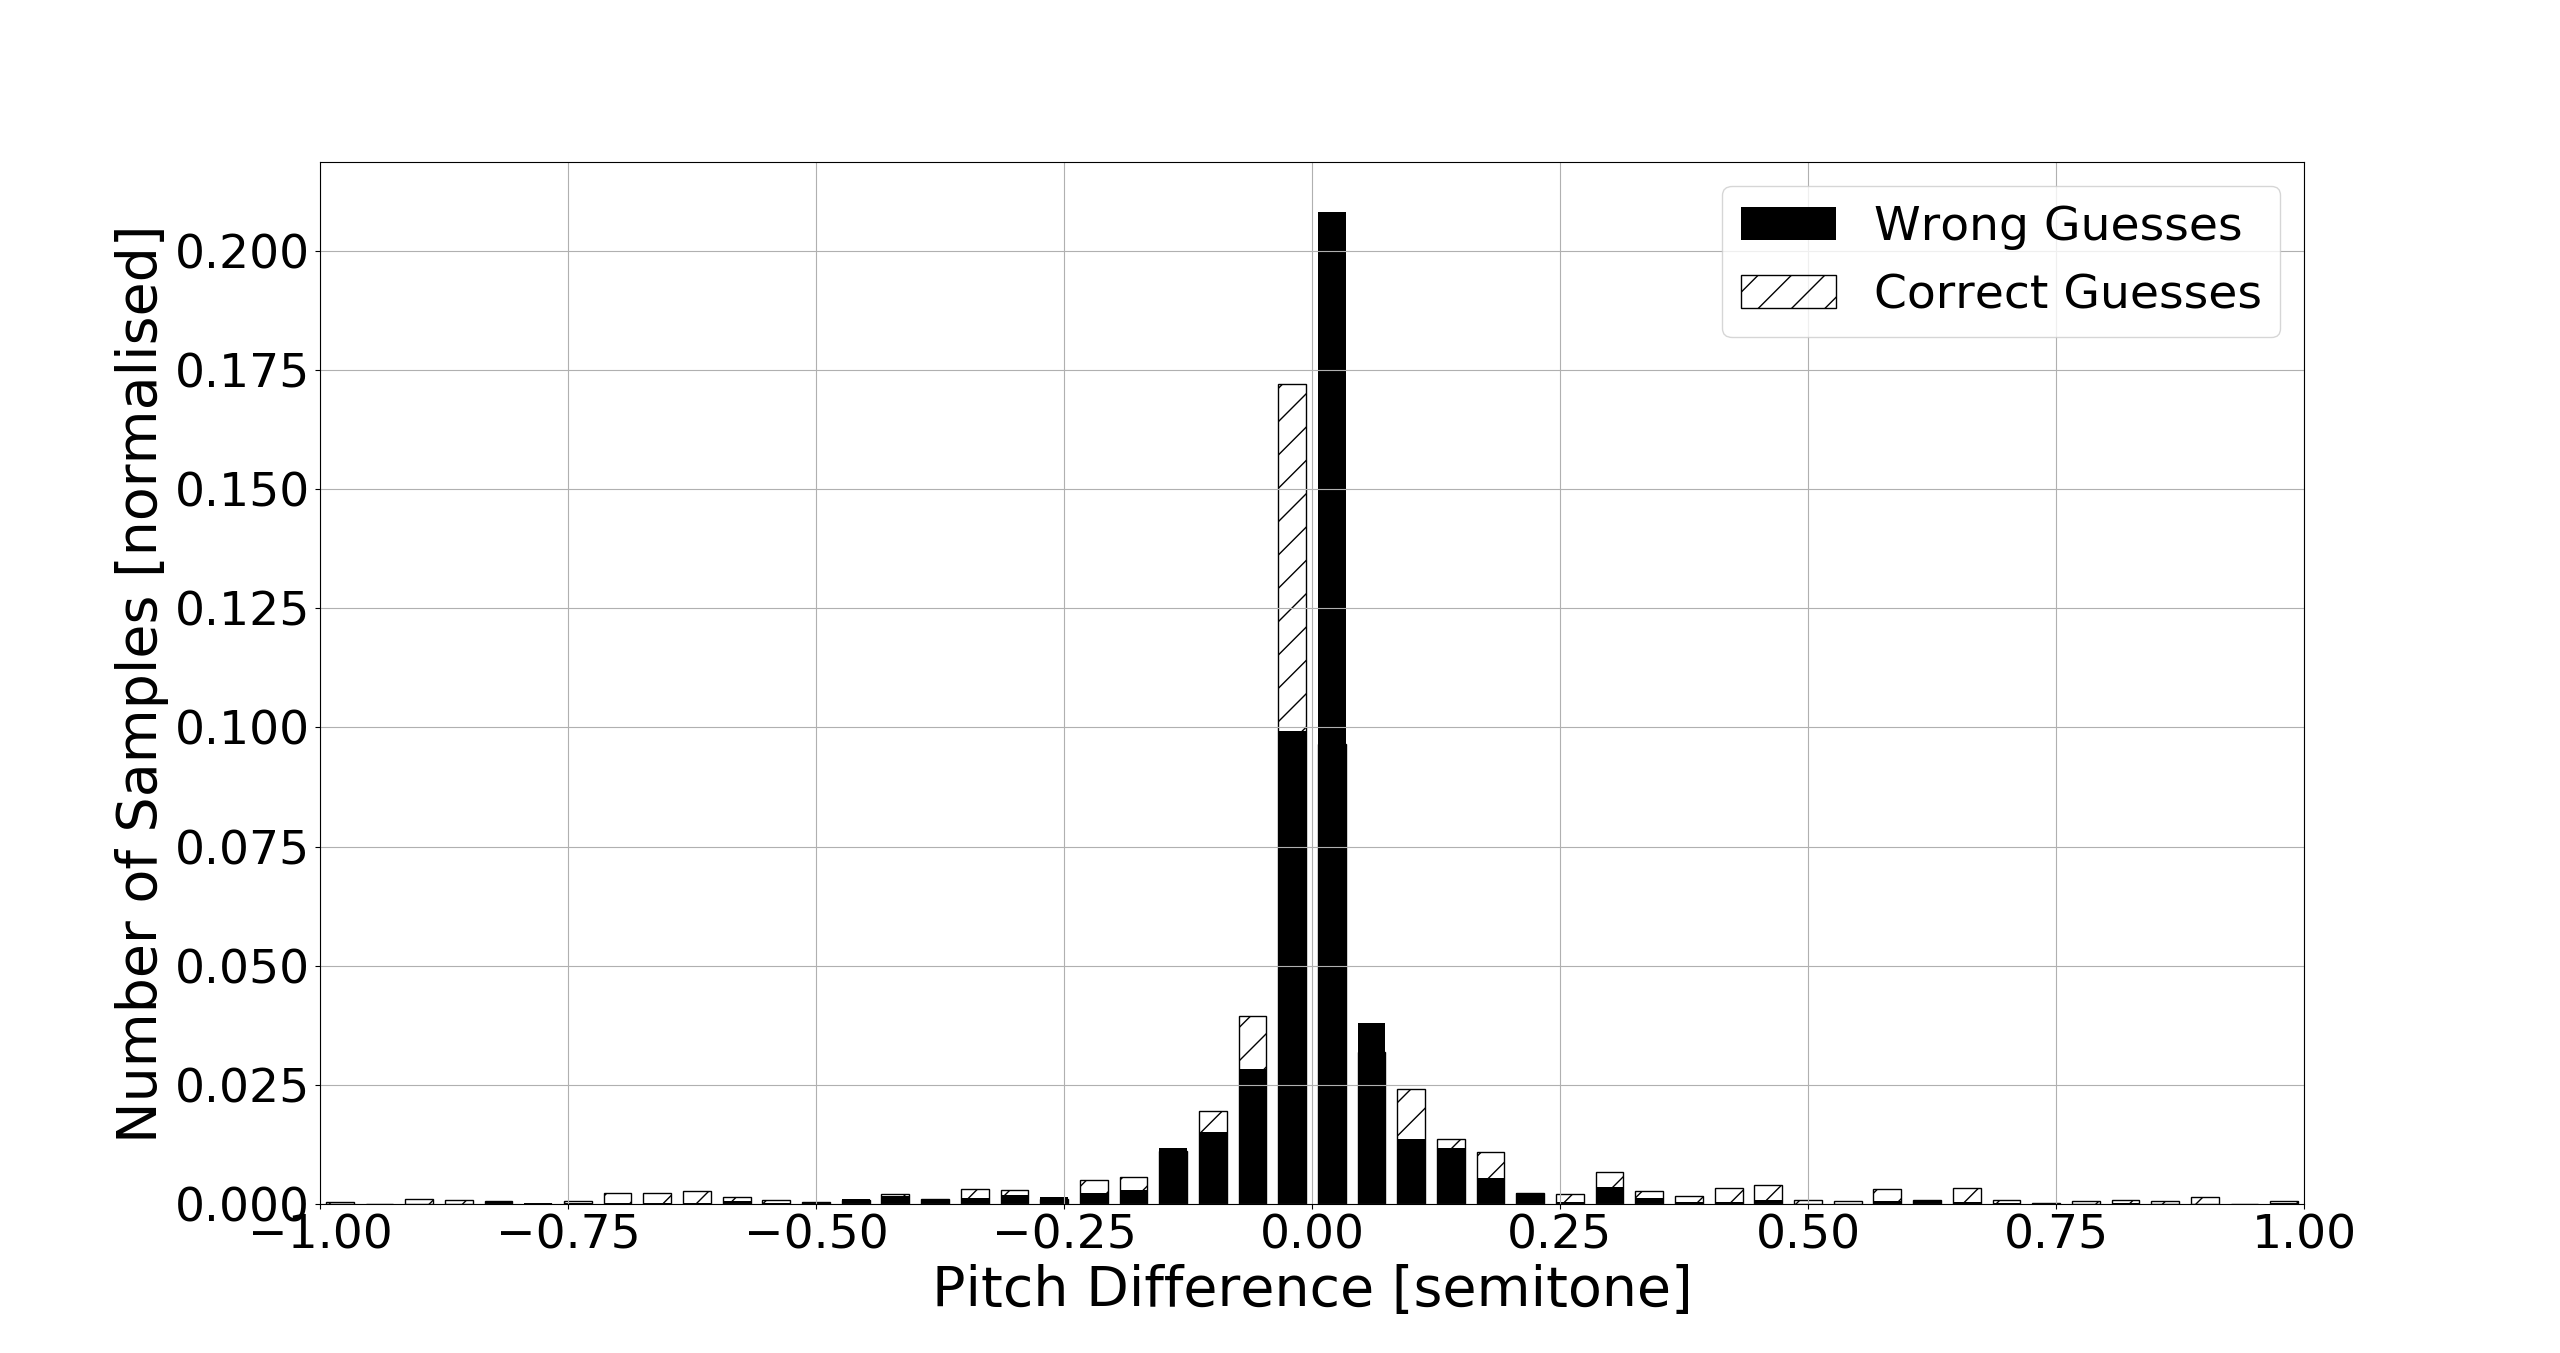
\includegraphics[clip, trim=80 0 150 100, width=0.4\textwidth]{figures/tone_guesses.png}
  %\caption{Results of the tone limit experiment. }
  %\label{fig:tone-guesses}
%\end{figure}

%\begin{figure}
  %\centering
  %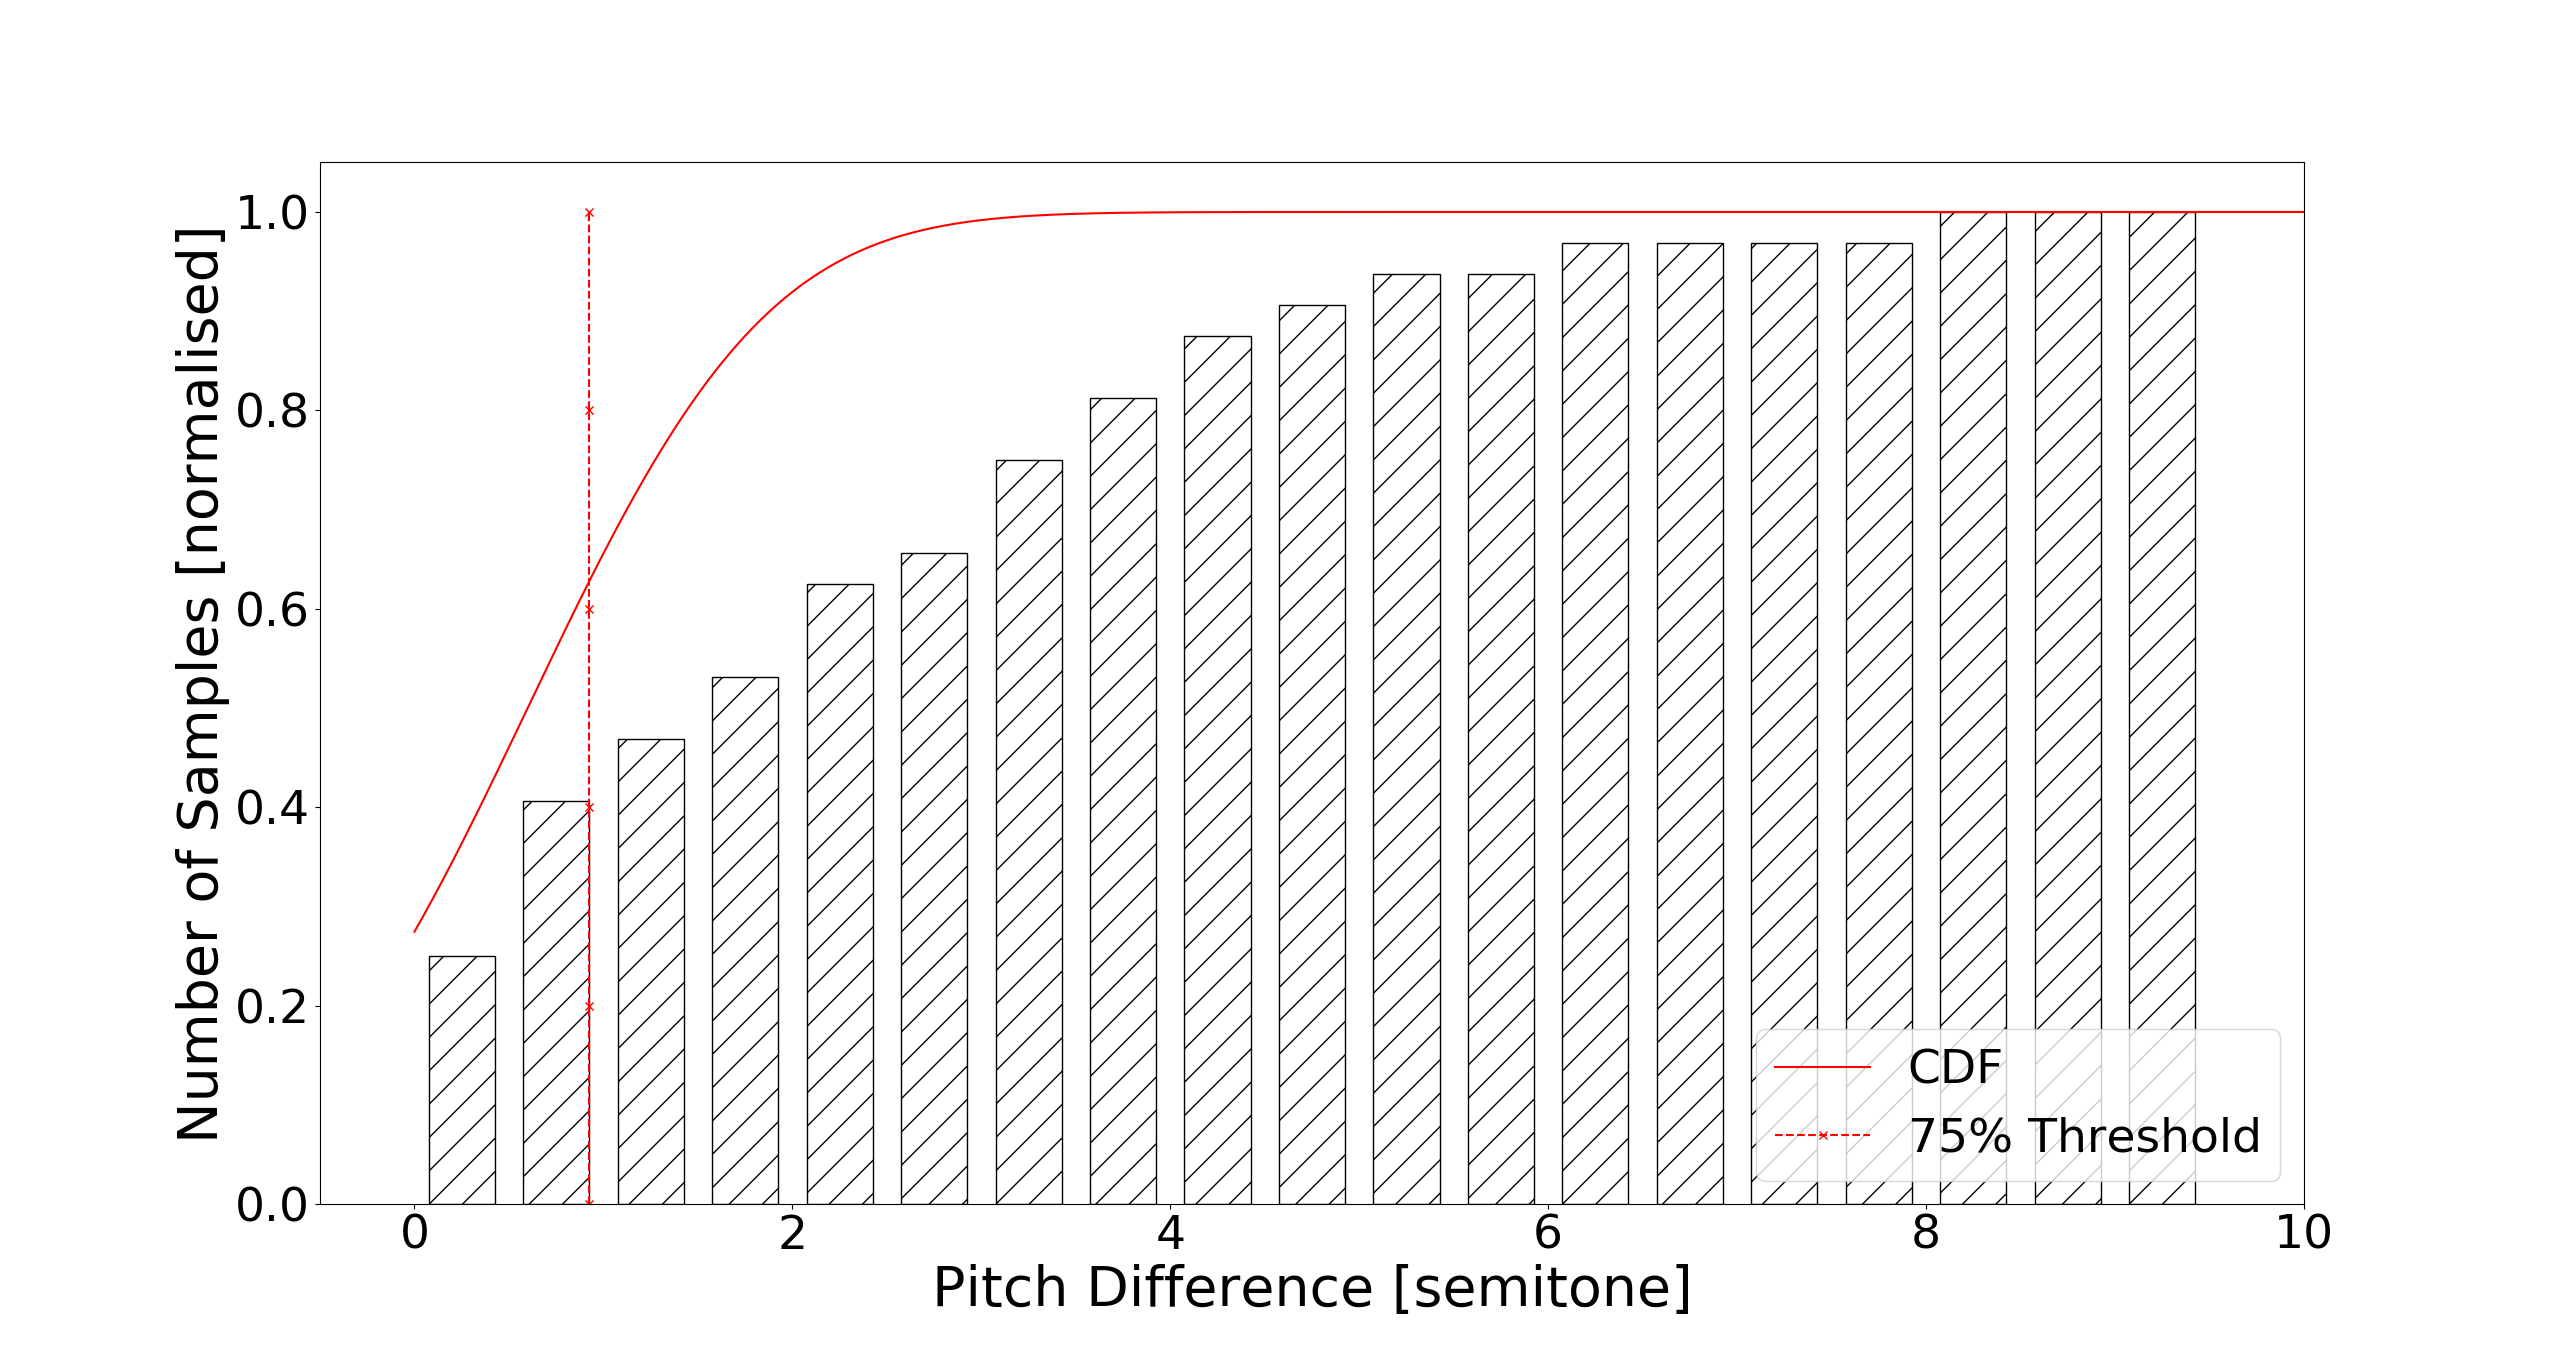
\includegraphics[clip, trim=120 0 120 70, width=0.4\textwidth]{figures/cdf_tone_guesses.png}
  %\caption{Cumulative distribution of the number of correct guesses for one participant. }
  %\label{fig:cdf-semitone}
%\end{figure}

%\begin{figure}
  %\centering
  %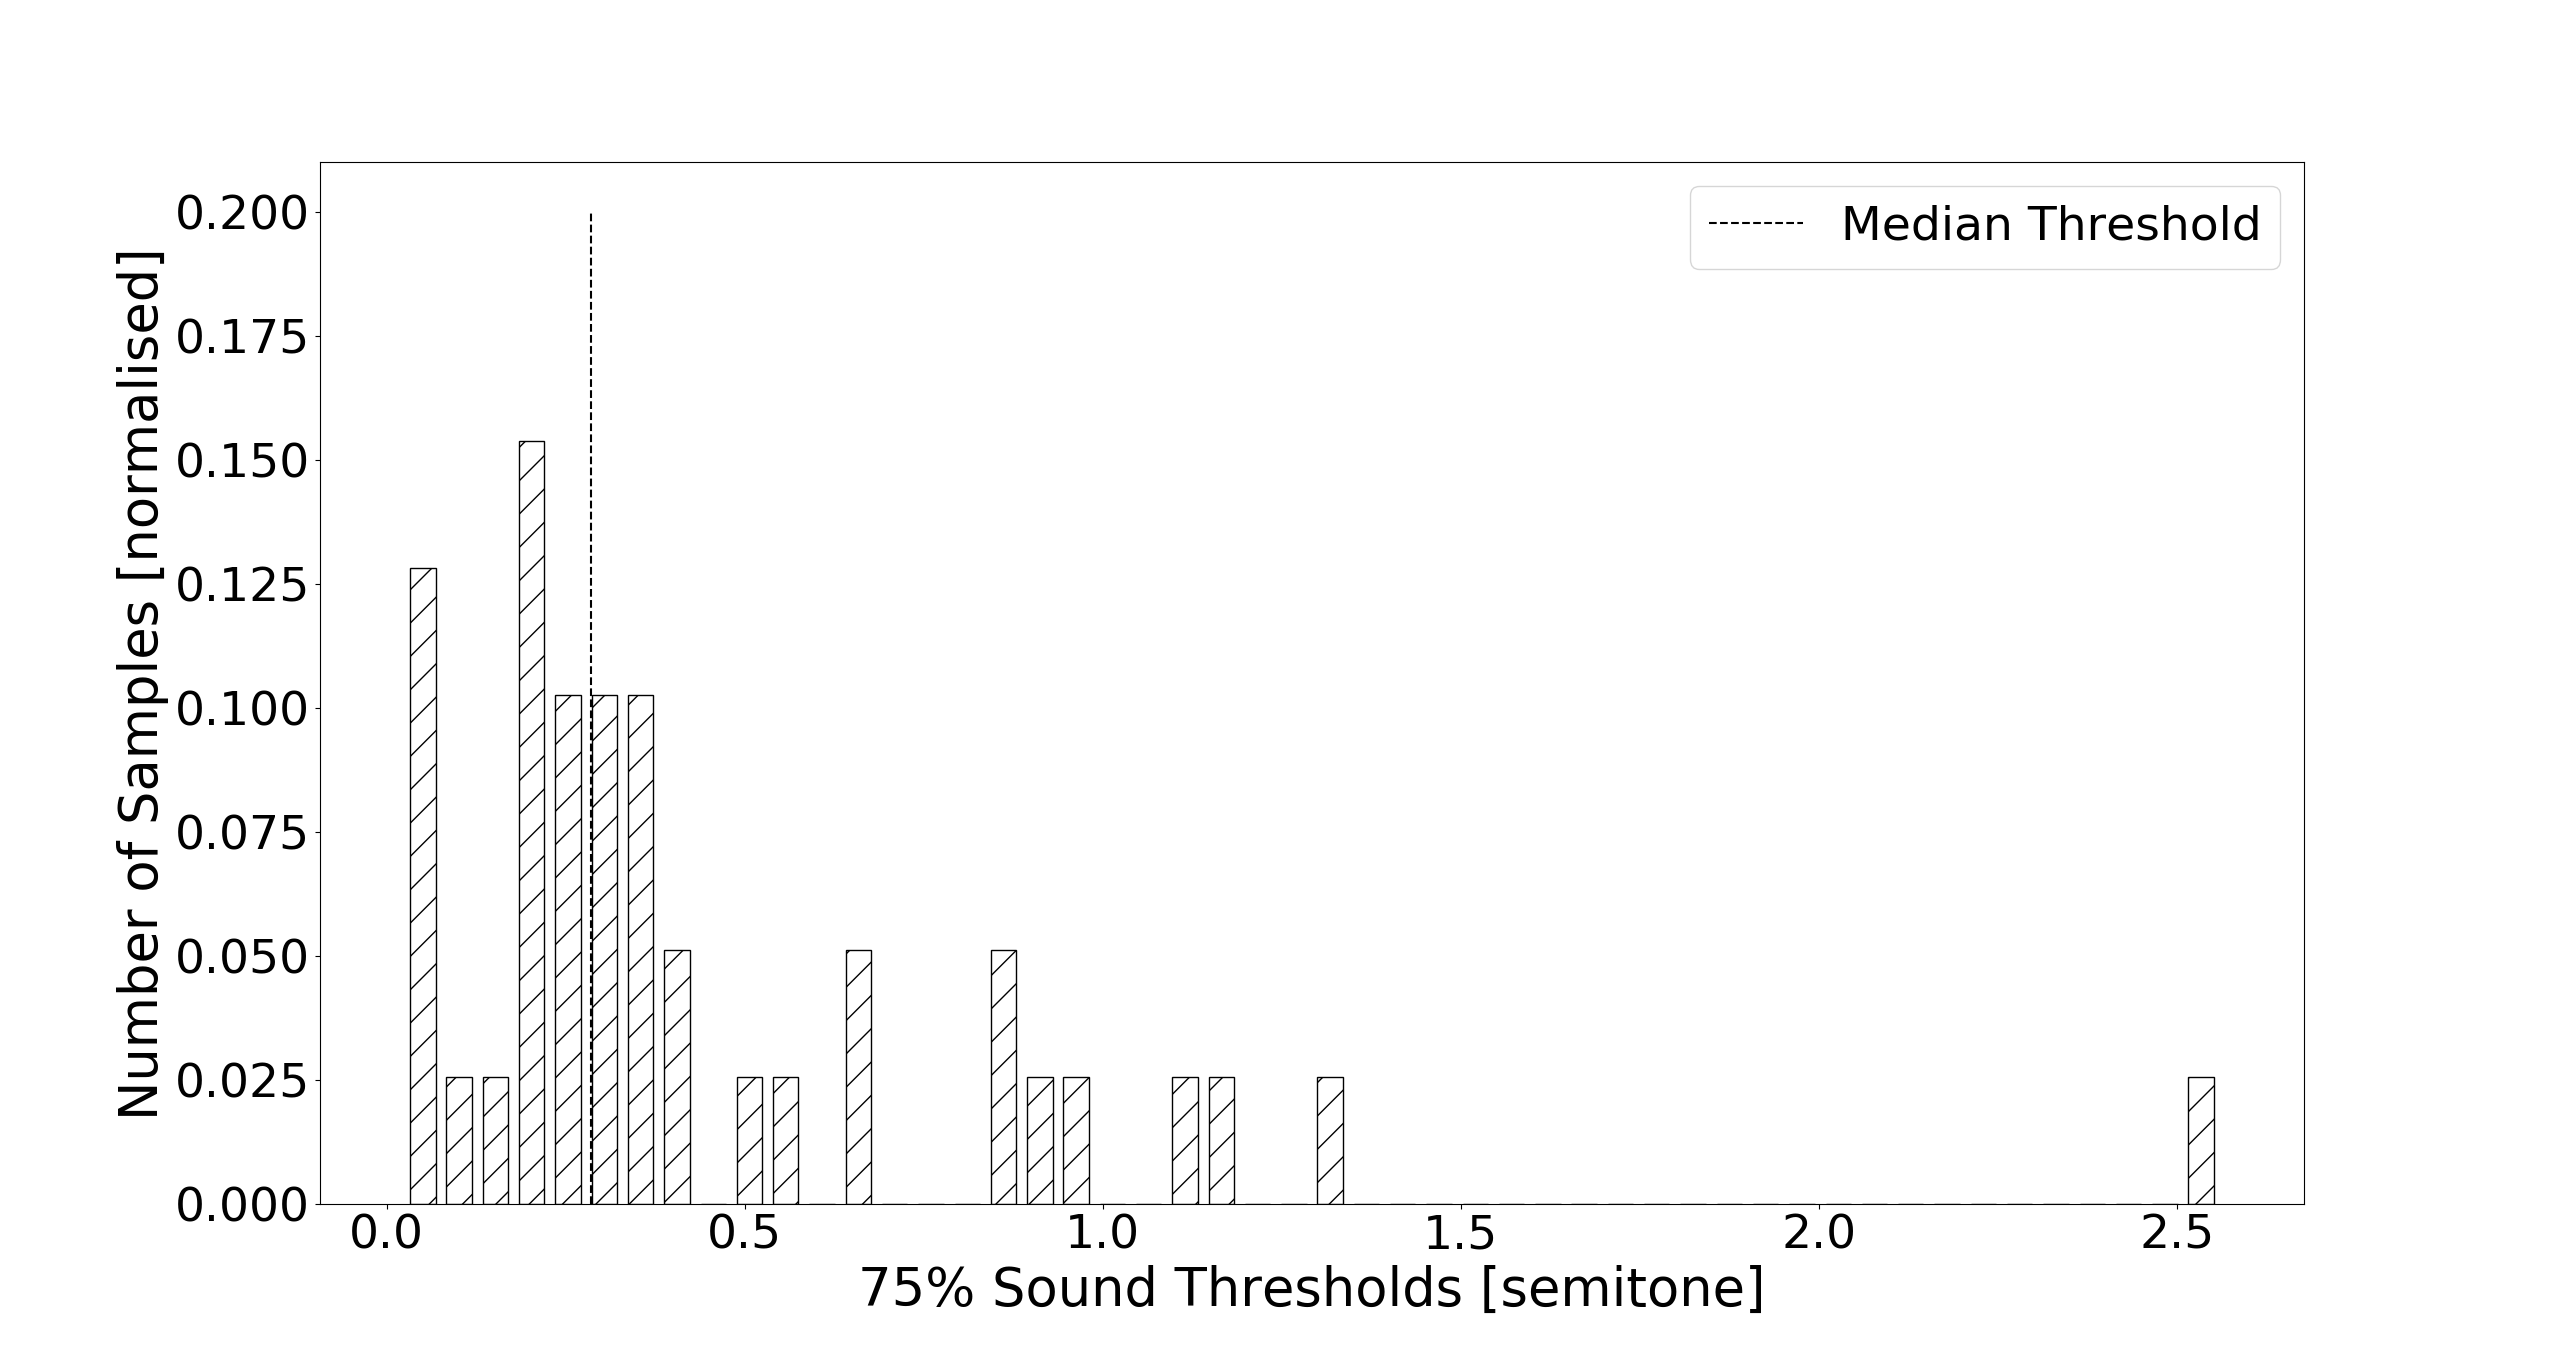
\includegraphics[clip, trim=80 20 120 0, width=0.4\textwidth]{figures/tone_threshold.png}
  %\caption{A distribution of the 75\% cut-off frequencies. }
  %\label{fig:tone-threshold}
%\end{figure}
%\begin{figure}
  %\centering
  %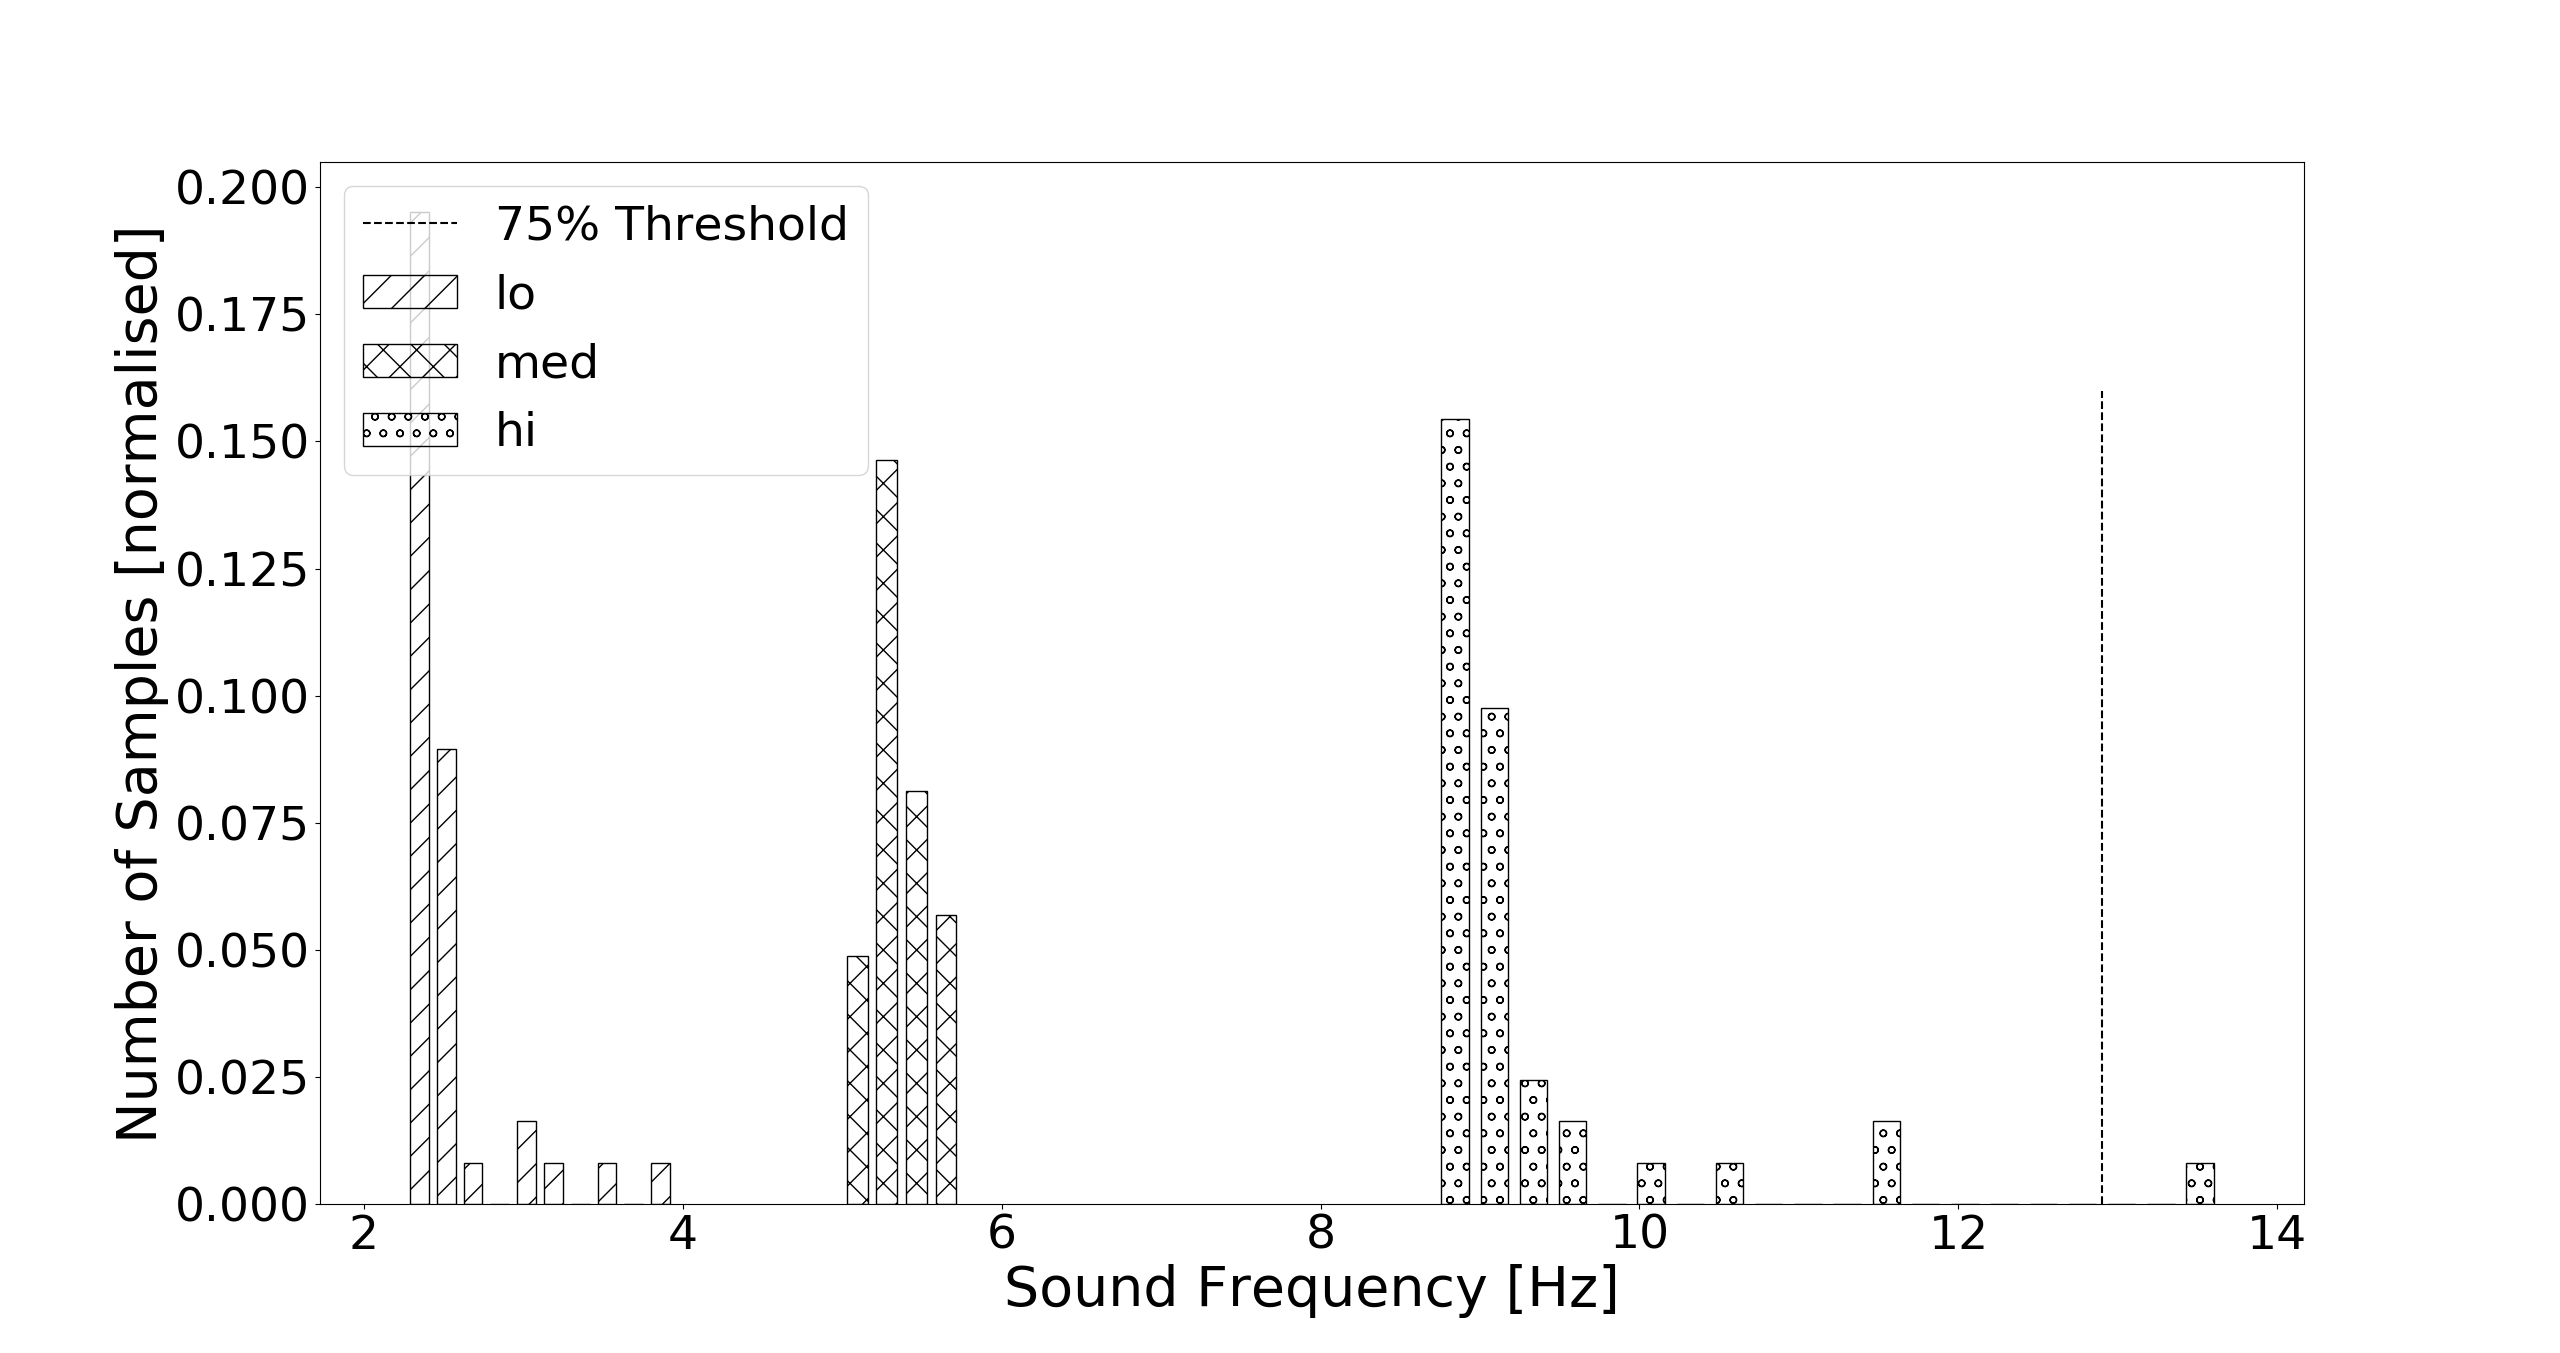
\includegraphics[clip, trim=80 20 120 0, width=0.4\textwidth]{figures/tone_medians.png}
  %\caption{A distribution of the median cut-off frequency thresholds along with the median 75\% cut-off threshold. }
  %\label{fig:tone-medians}
%\end{figure}

%\subsection{Target Search}

\subsection{Panning Results}

The results from the target search experiment in the pan dimension are given on the abscissa of the 2D histograms in \crefrange{fig:err-results-lo}{fig:err-results-hi}, where the angular errors in the pan and tilt directions are plotted against each other.
A set of box-plots of the pan errors' median and standard deviations are also given in \crefrange{fig:err-boxplot-median}{fig:err-boxplot-std} for each of the \emph{lo}, \emph{med} and \emph{hi} configurations.
The results are summarised in Table~\ref{tab:results}.

\begin{figure}
  \centering
  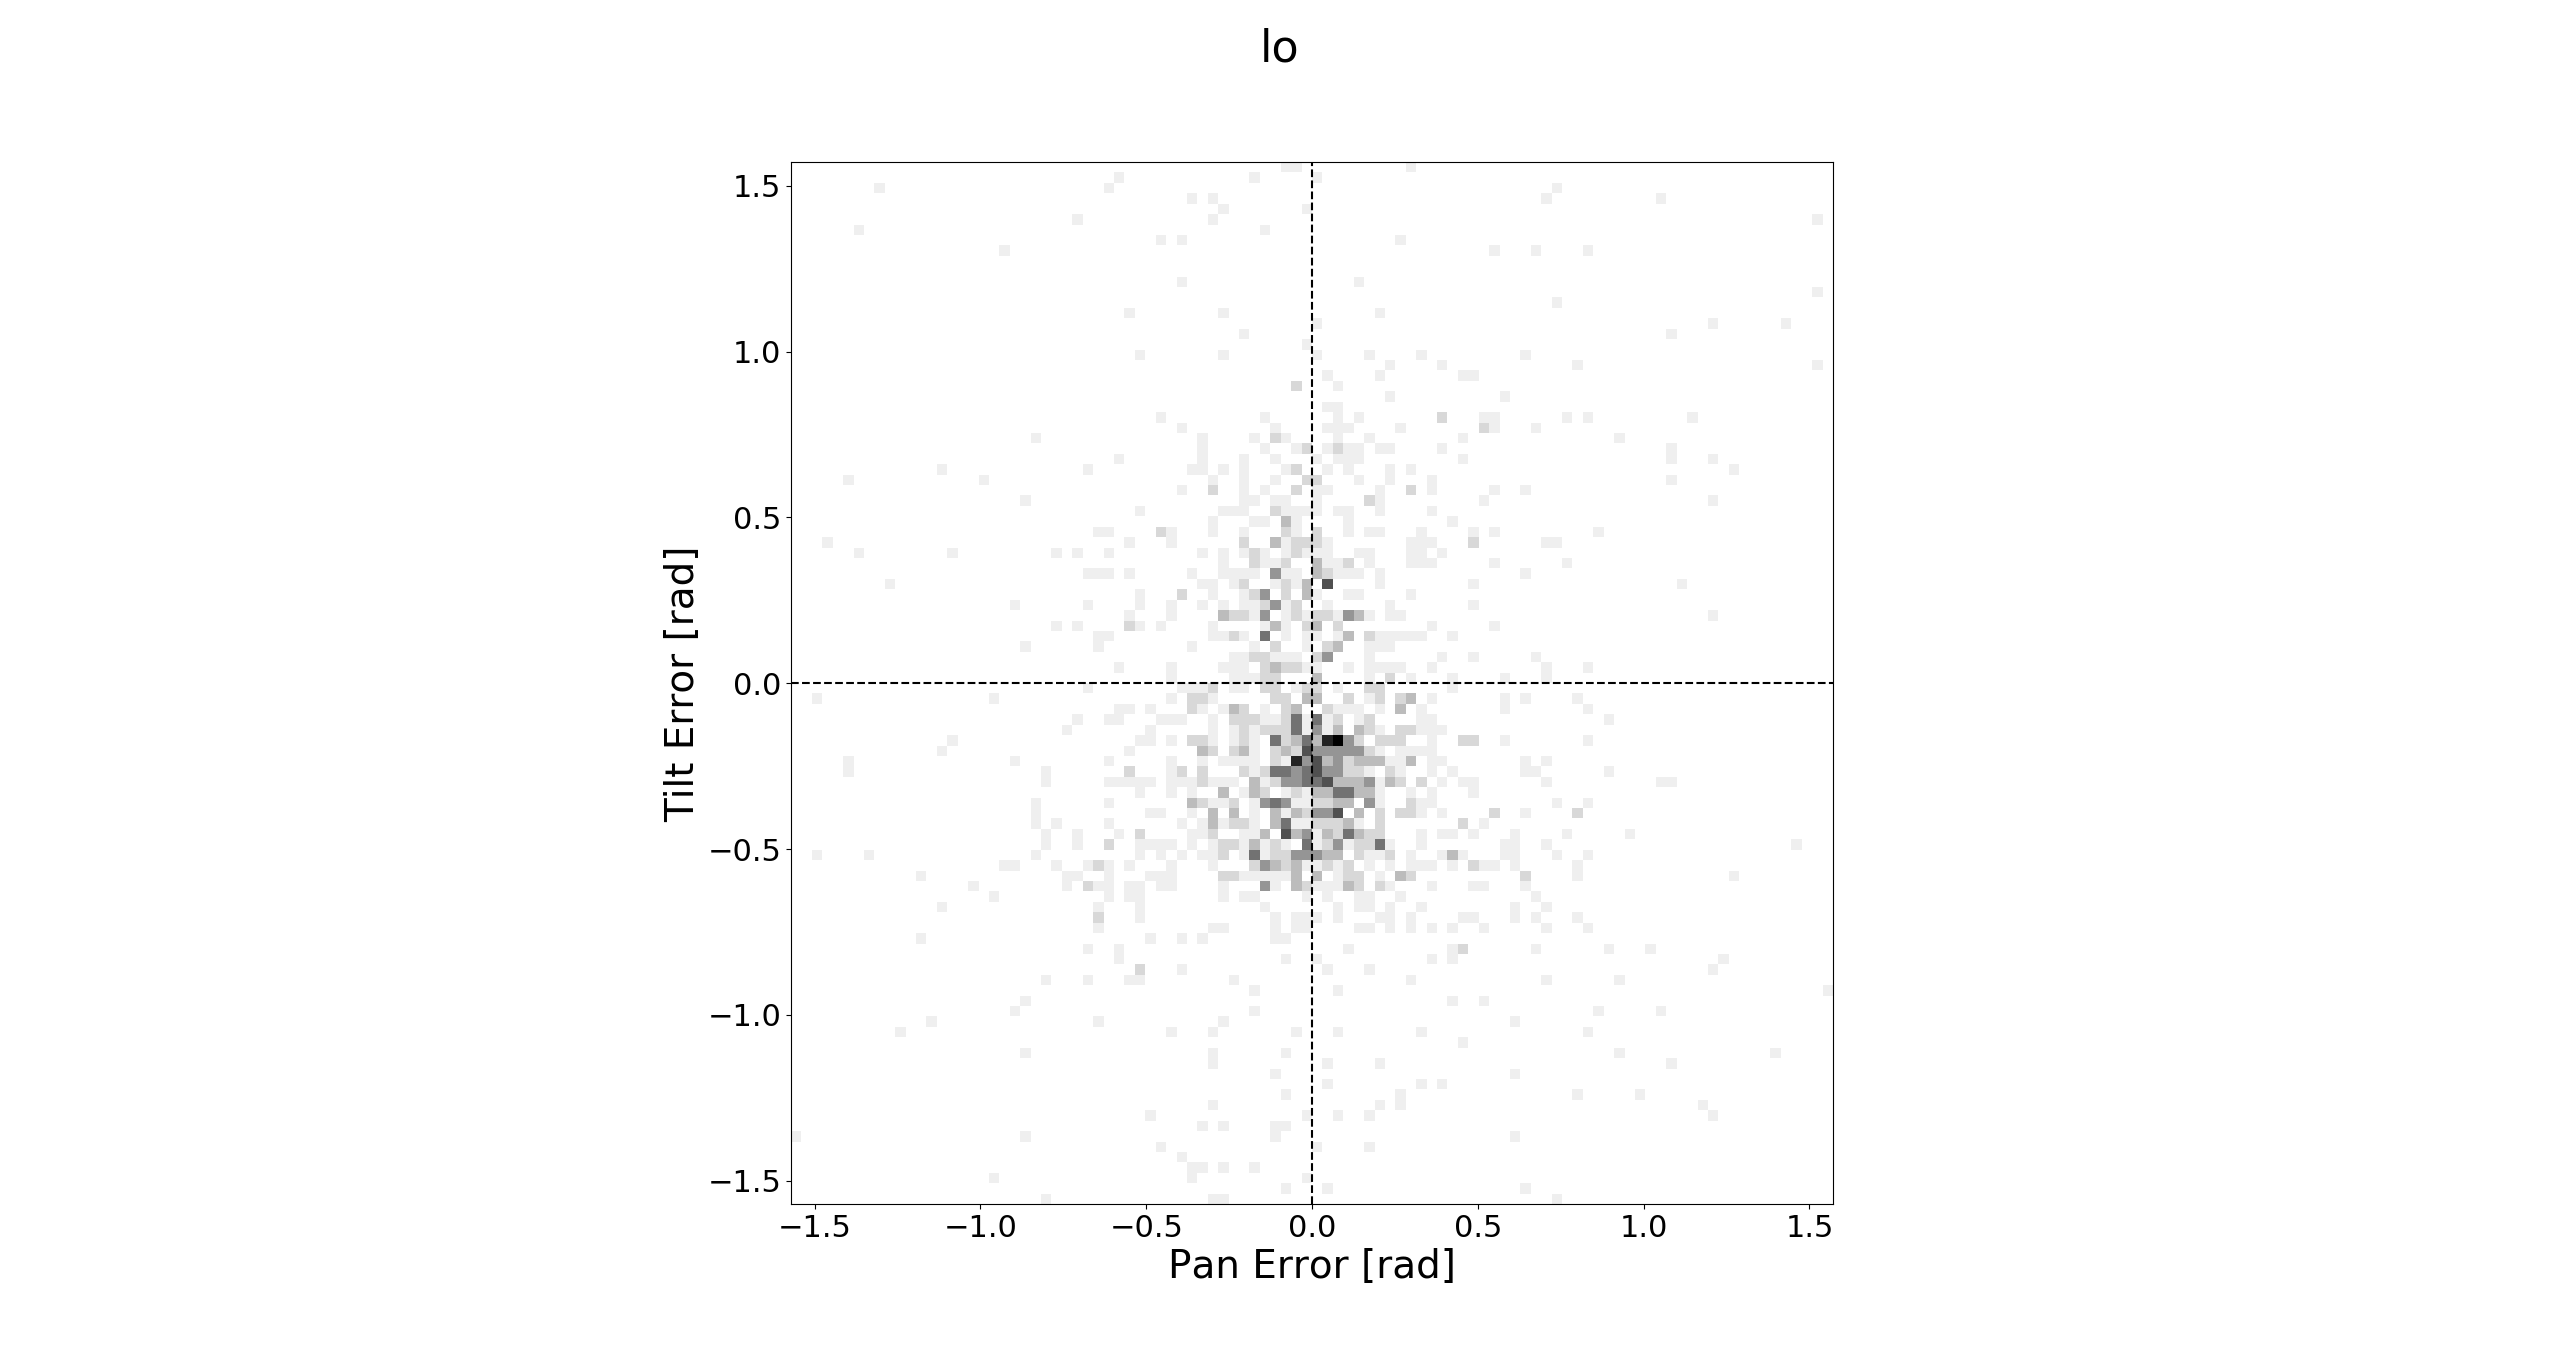
\includegraphics[clip, trim=450 0 450 110, width=0.4\textwidth]{figures/err_lo.png}
  \caption{\emph{Lo} setting. }
  \label{fig:err-results-lo}
\end{figure}
\begin{figure}
  \centering
  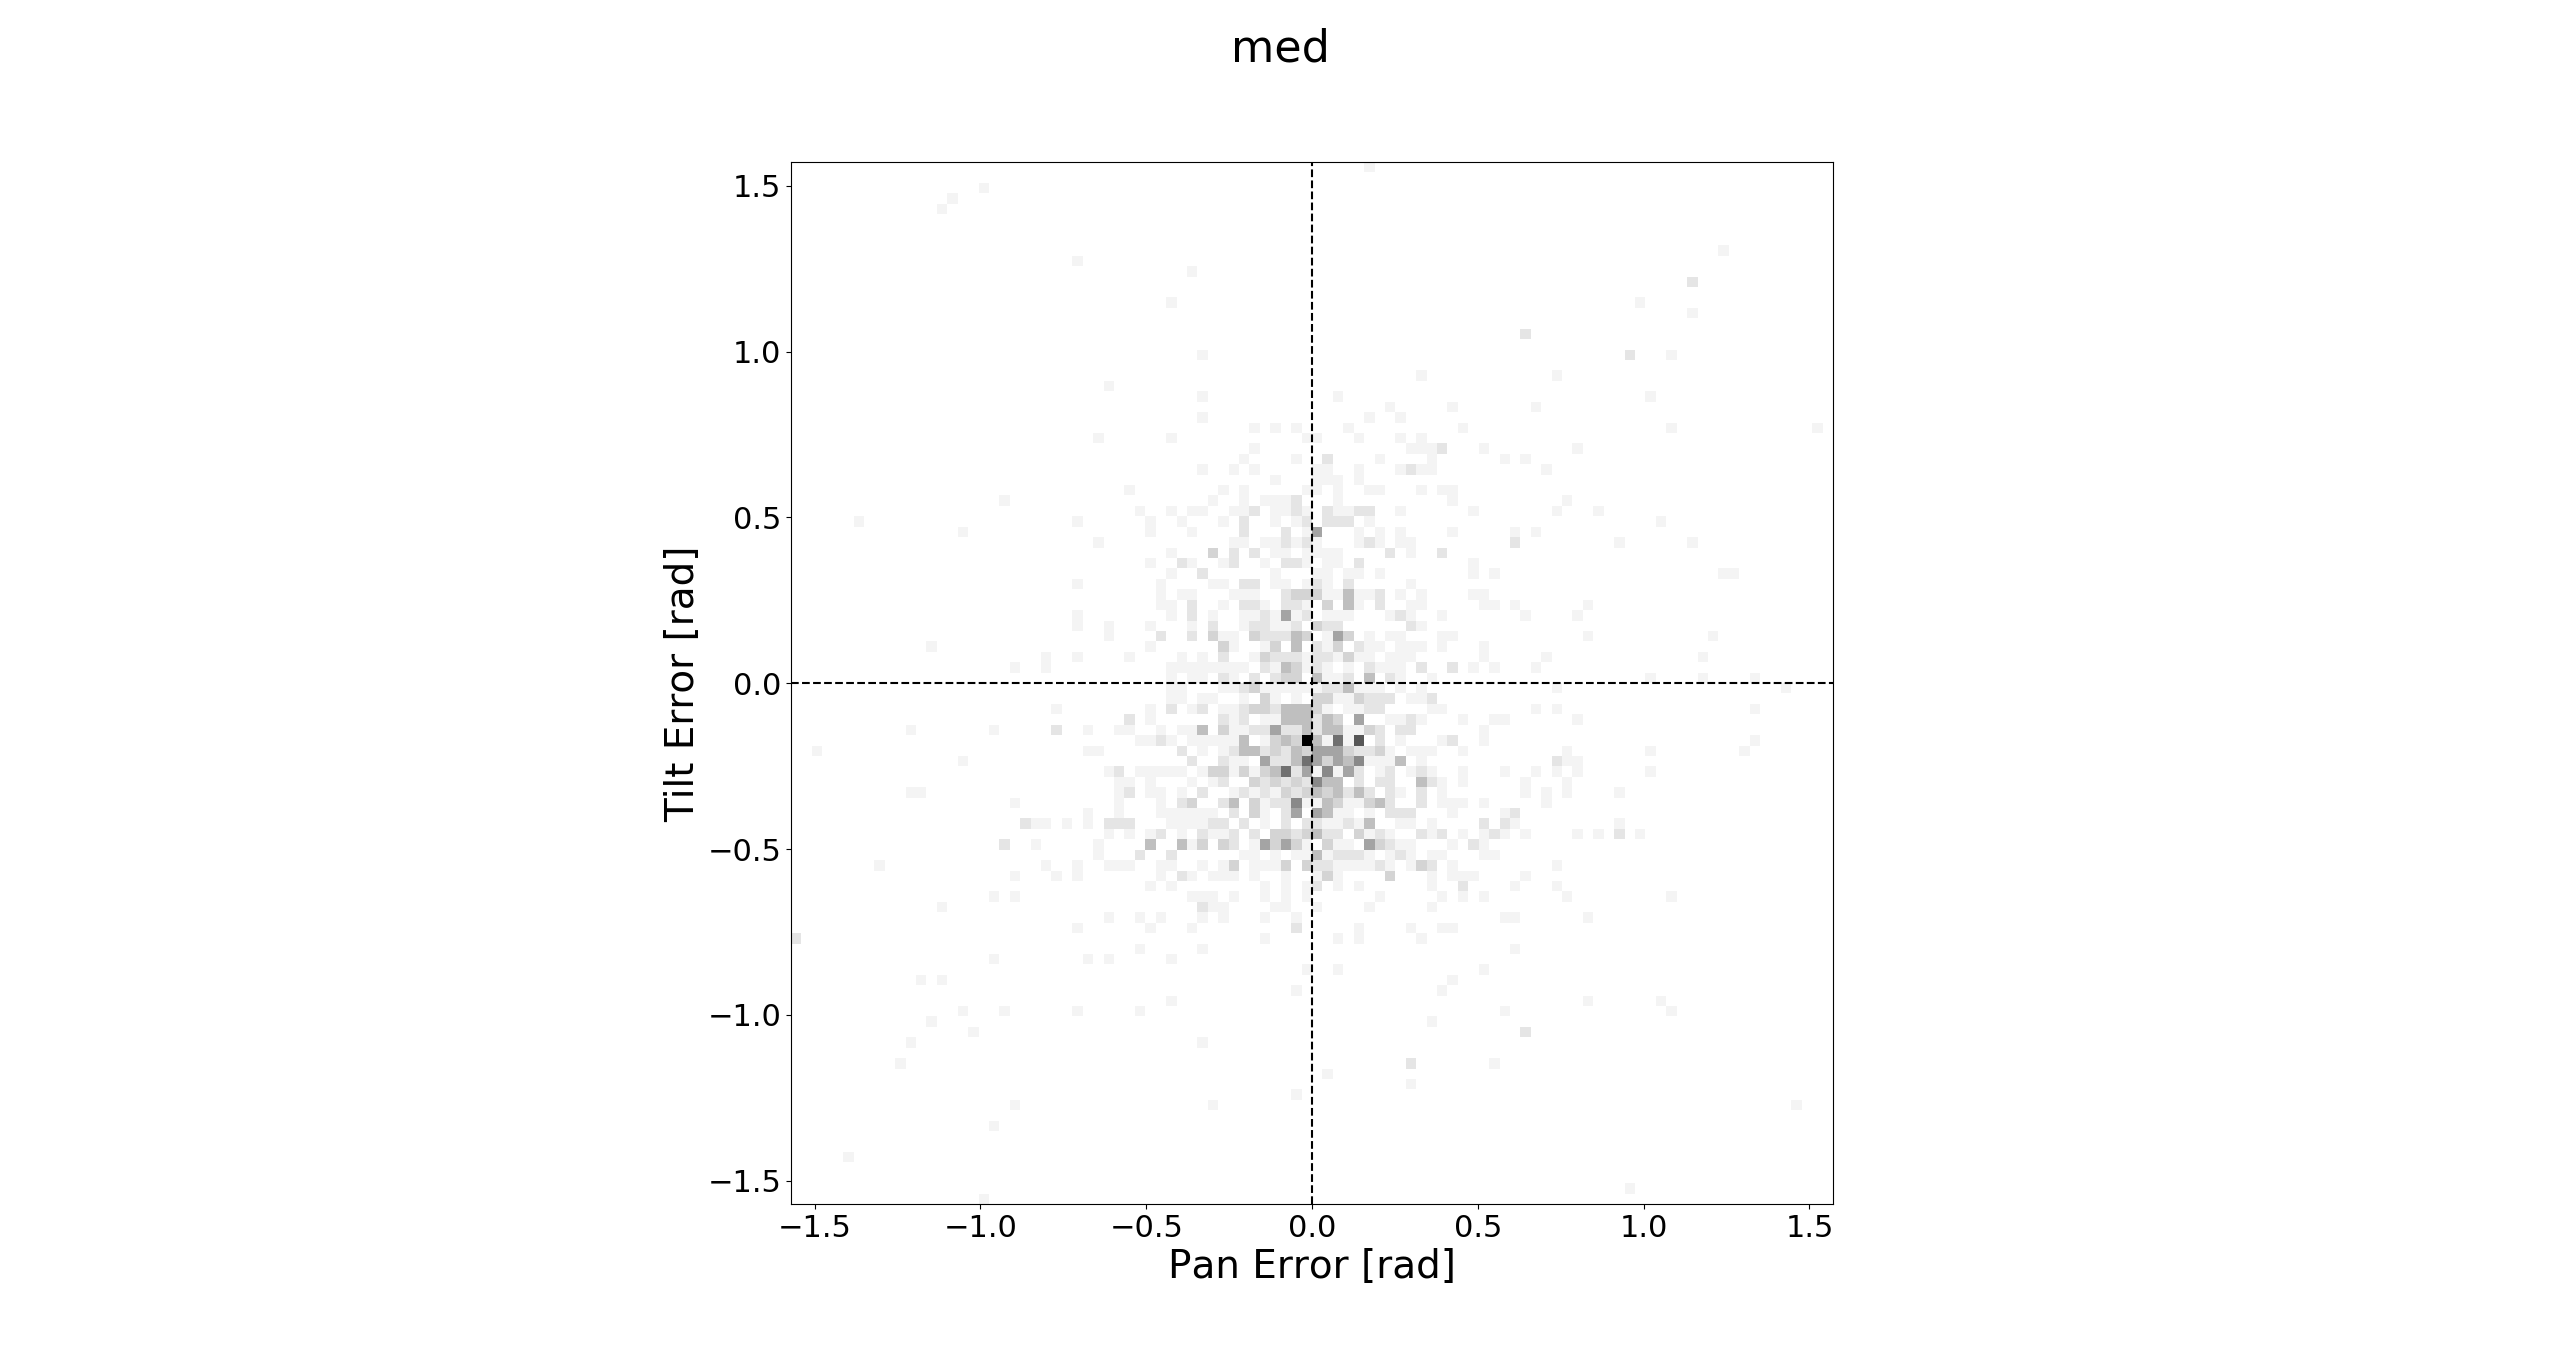
\includegraphics[clip, trim=450 0 450 110, width=0.4\textwidth]{figures/err_med.png}
  \caption{\emph{Med} setting. }
  \label{fig:err-results-med}
\end{figure}

\begin{figure}
  \centering
  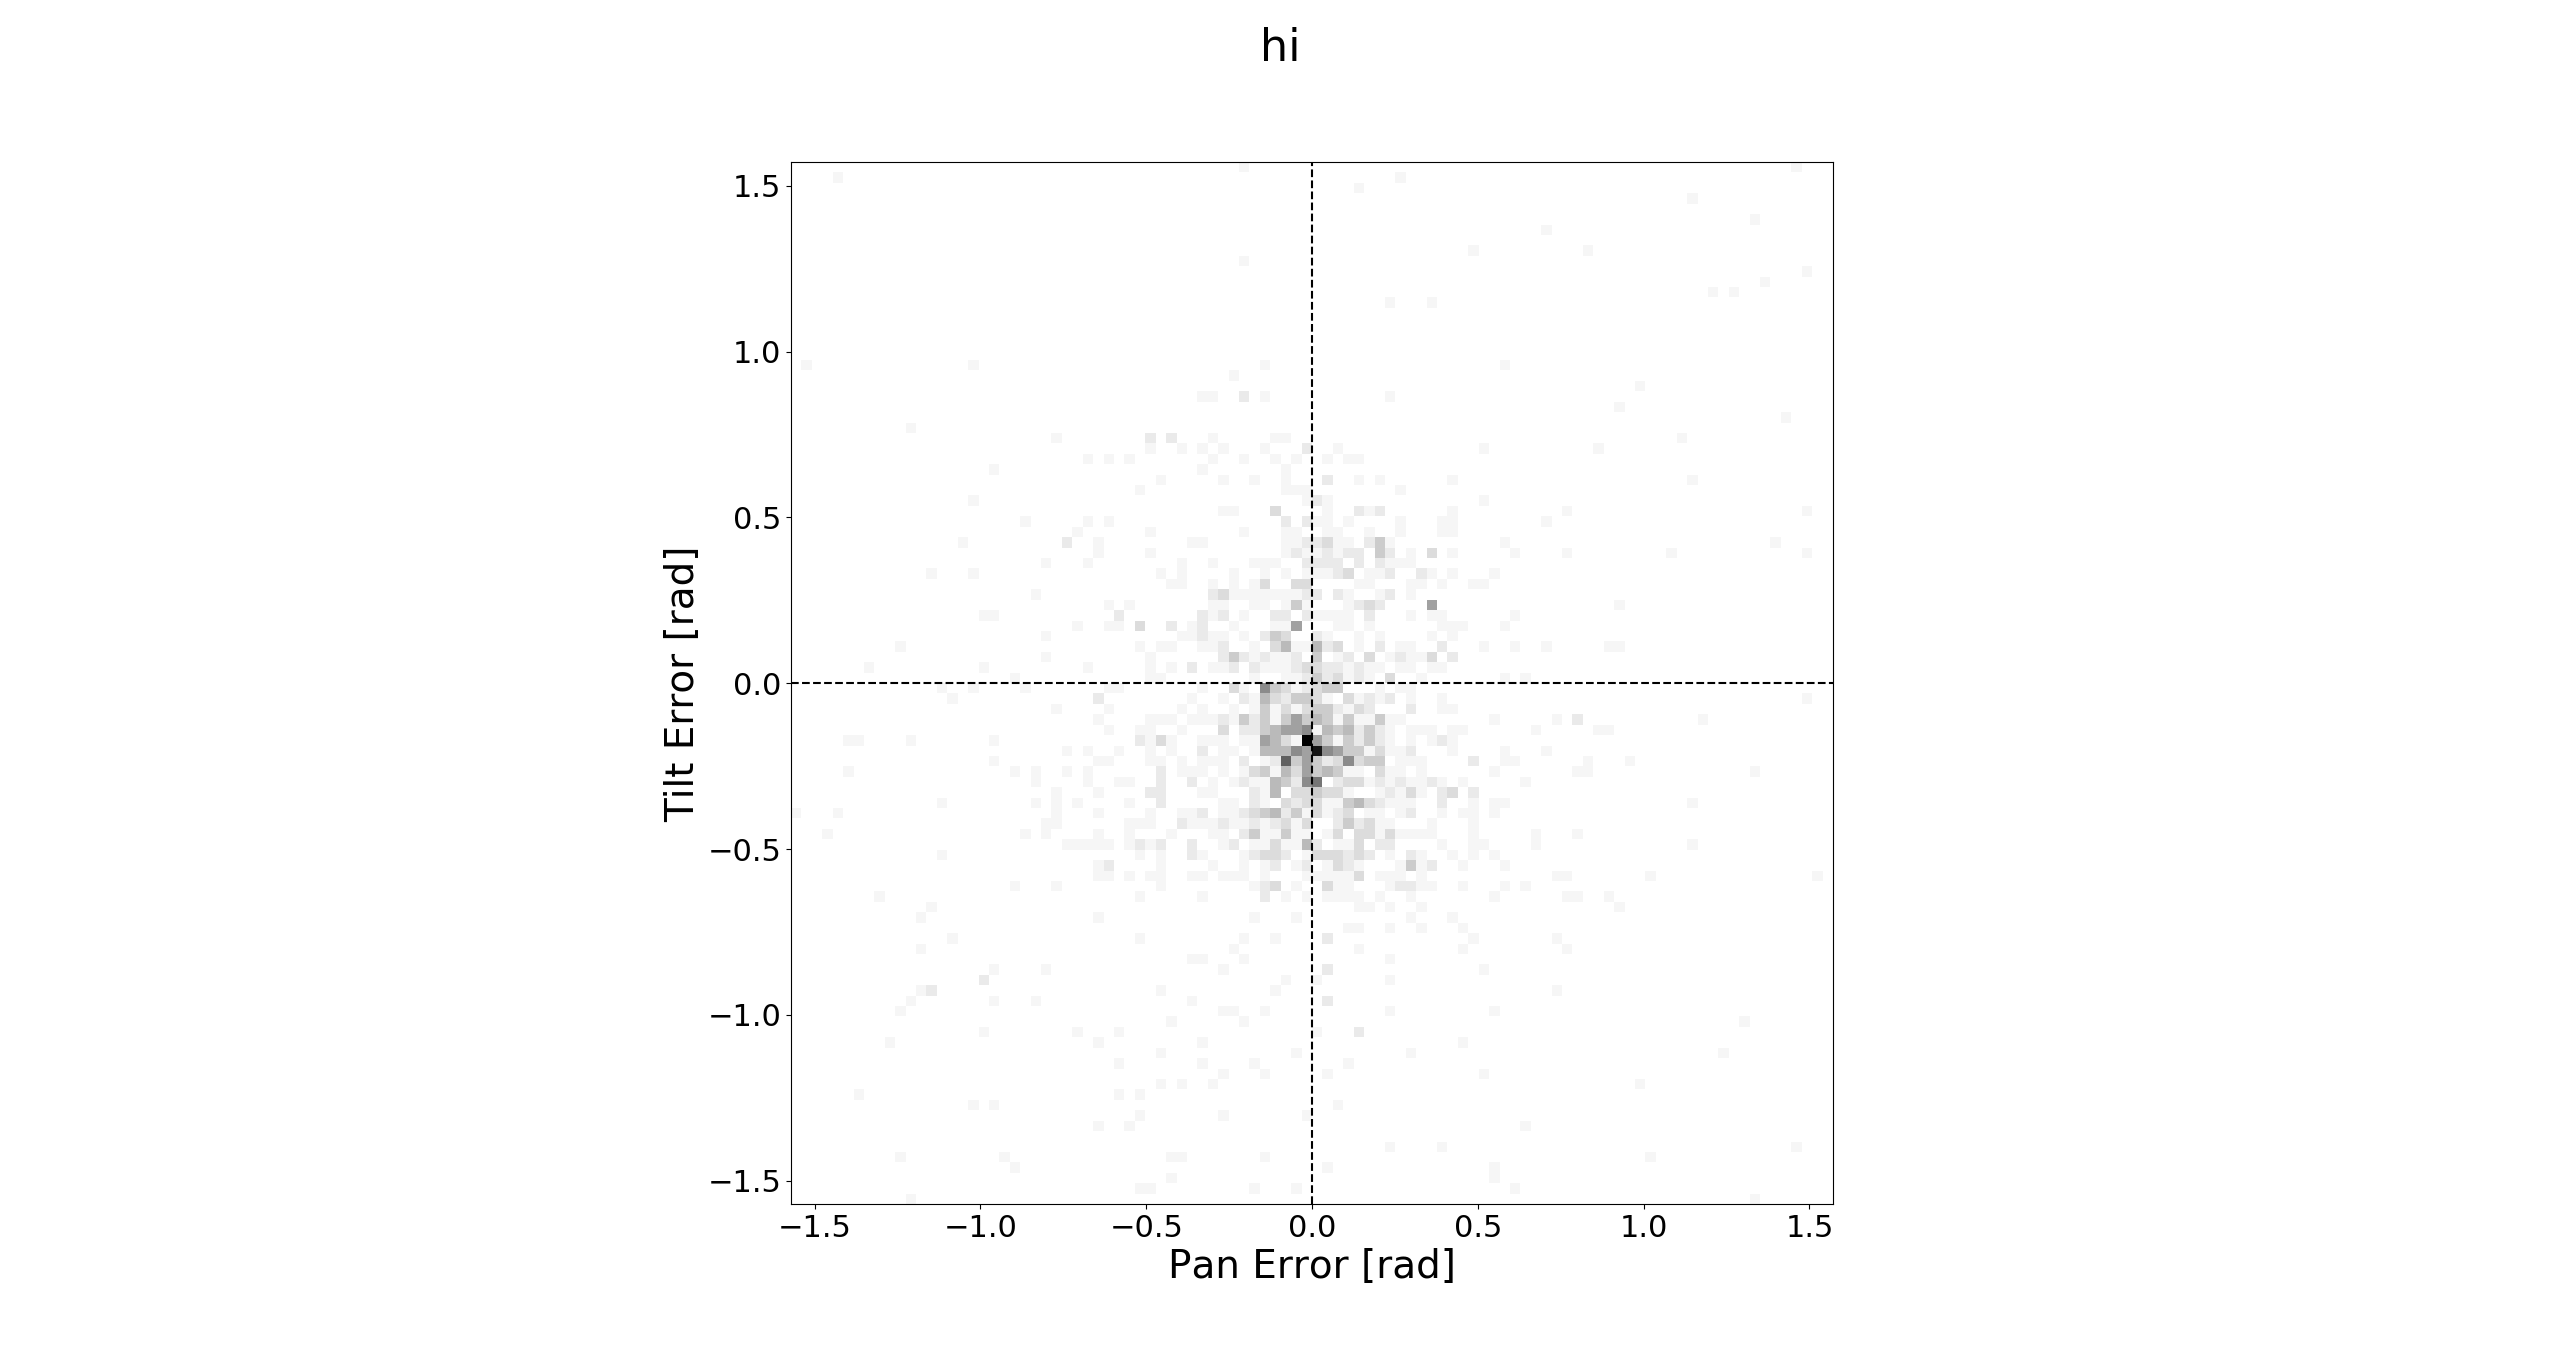
\includegraphics[clip, trim=450 0 450 60, width=0.4\textwidth]{figures/err_hi.png}
  \caption{\emph{Hi} setting. }
  \label{fig:err-results-hi}
\end{figure}

\begin{figure}
  \centering
  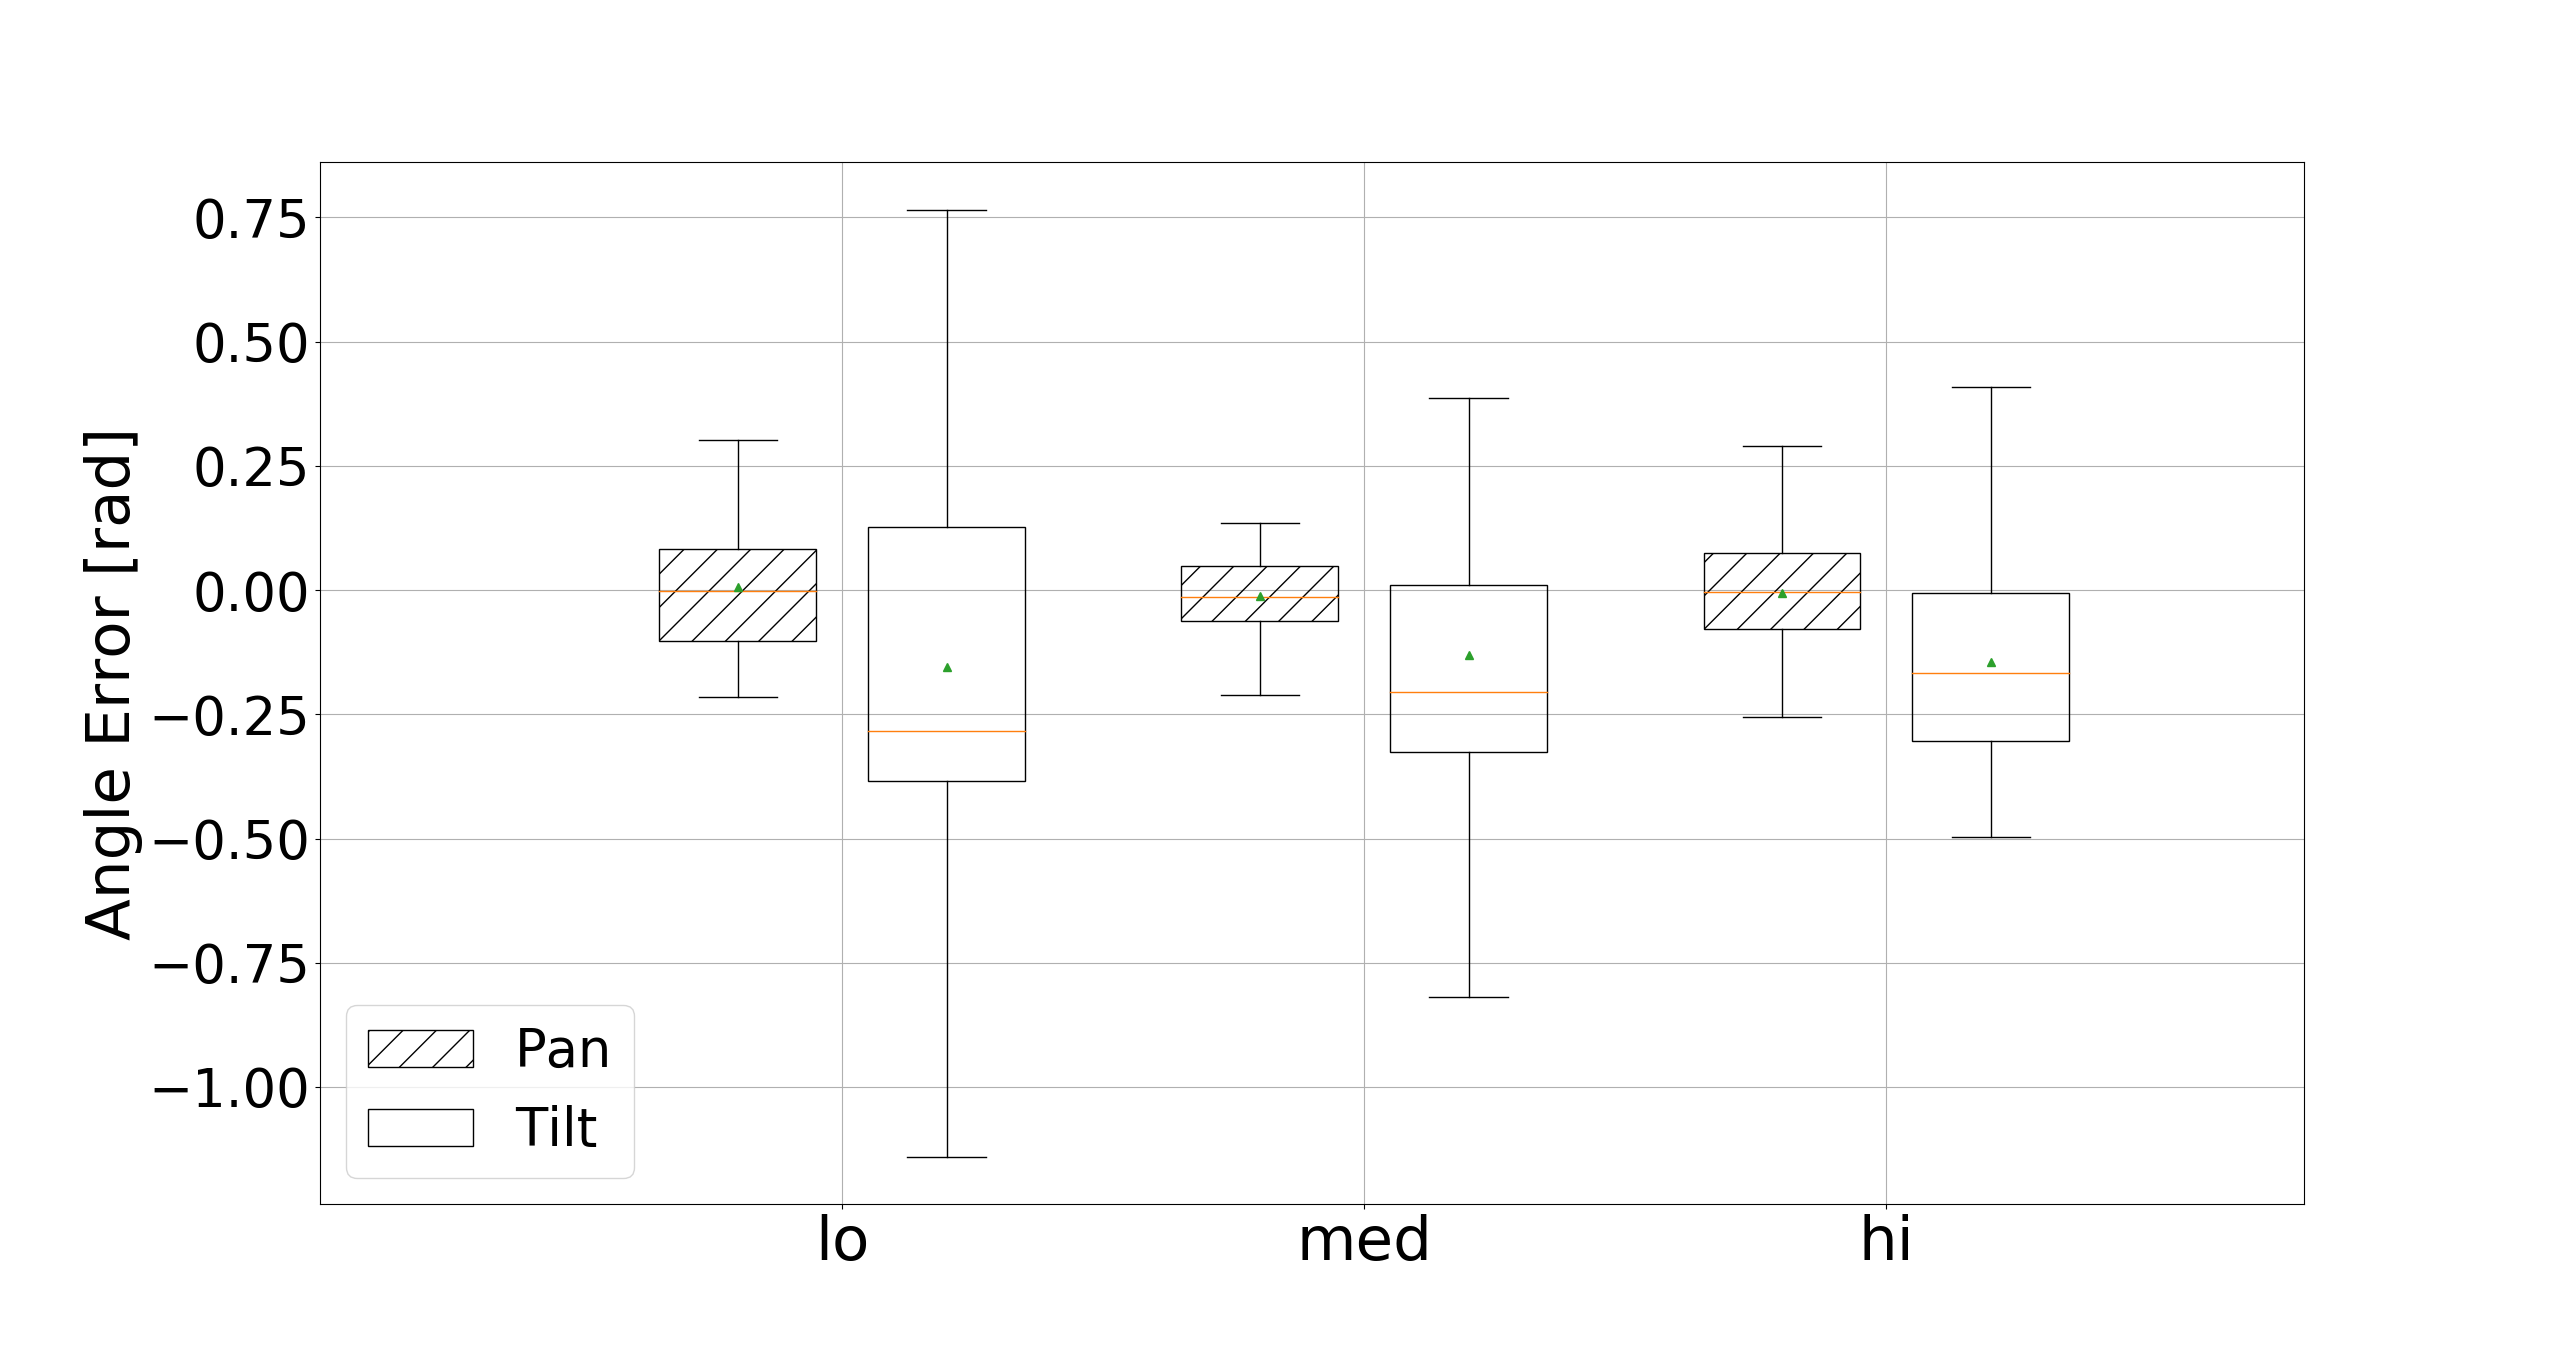
\includegraphics[clip, trim=20 -70 100 100, width=0.4\textwidth]{figures/err_boxplot_medians.png}
  \caption{Error median.}
  \label{fig:err-boxplot-median}
\end{figure}

\begin{figure}
  \centering
  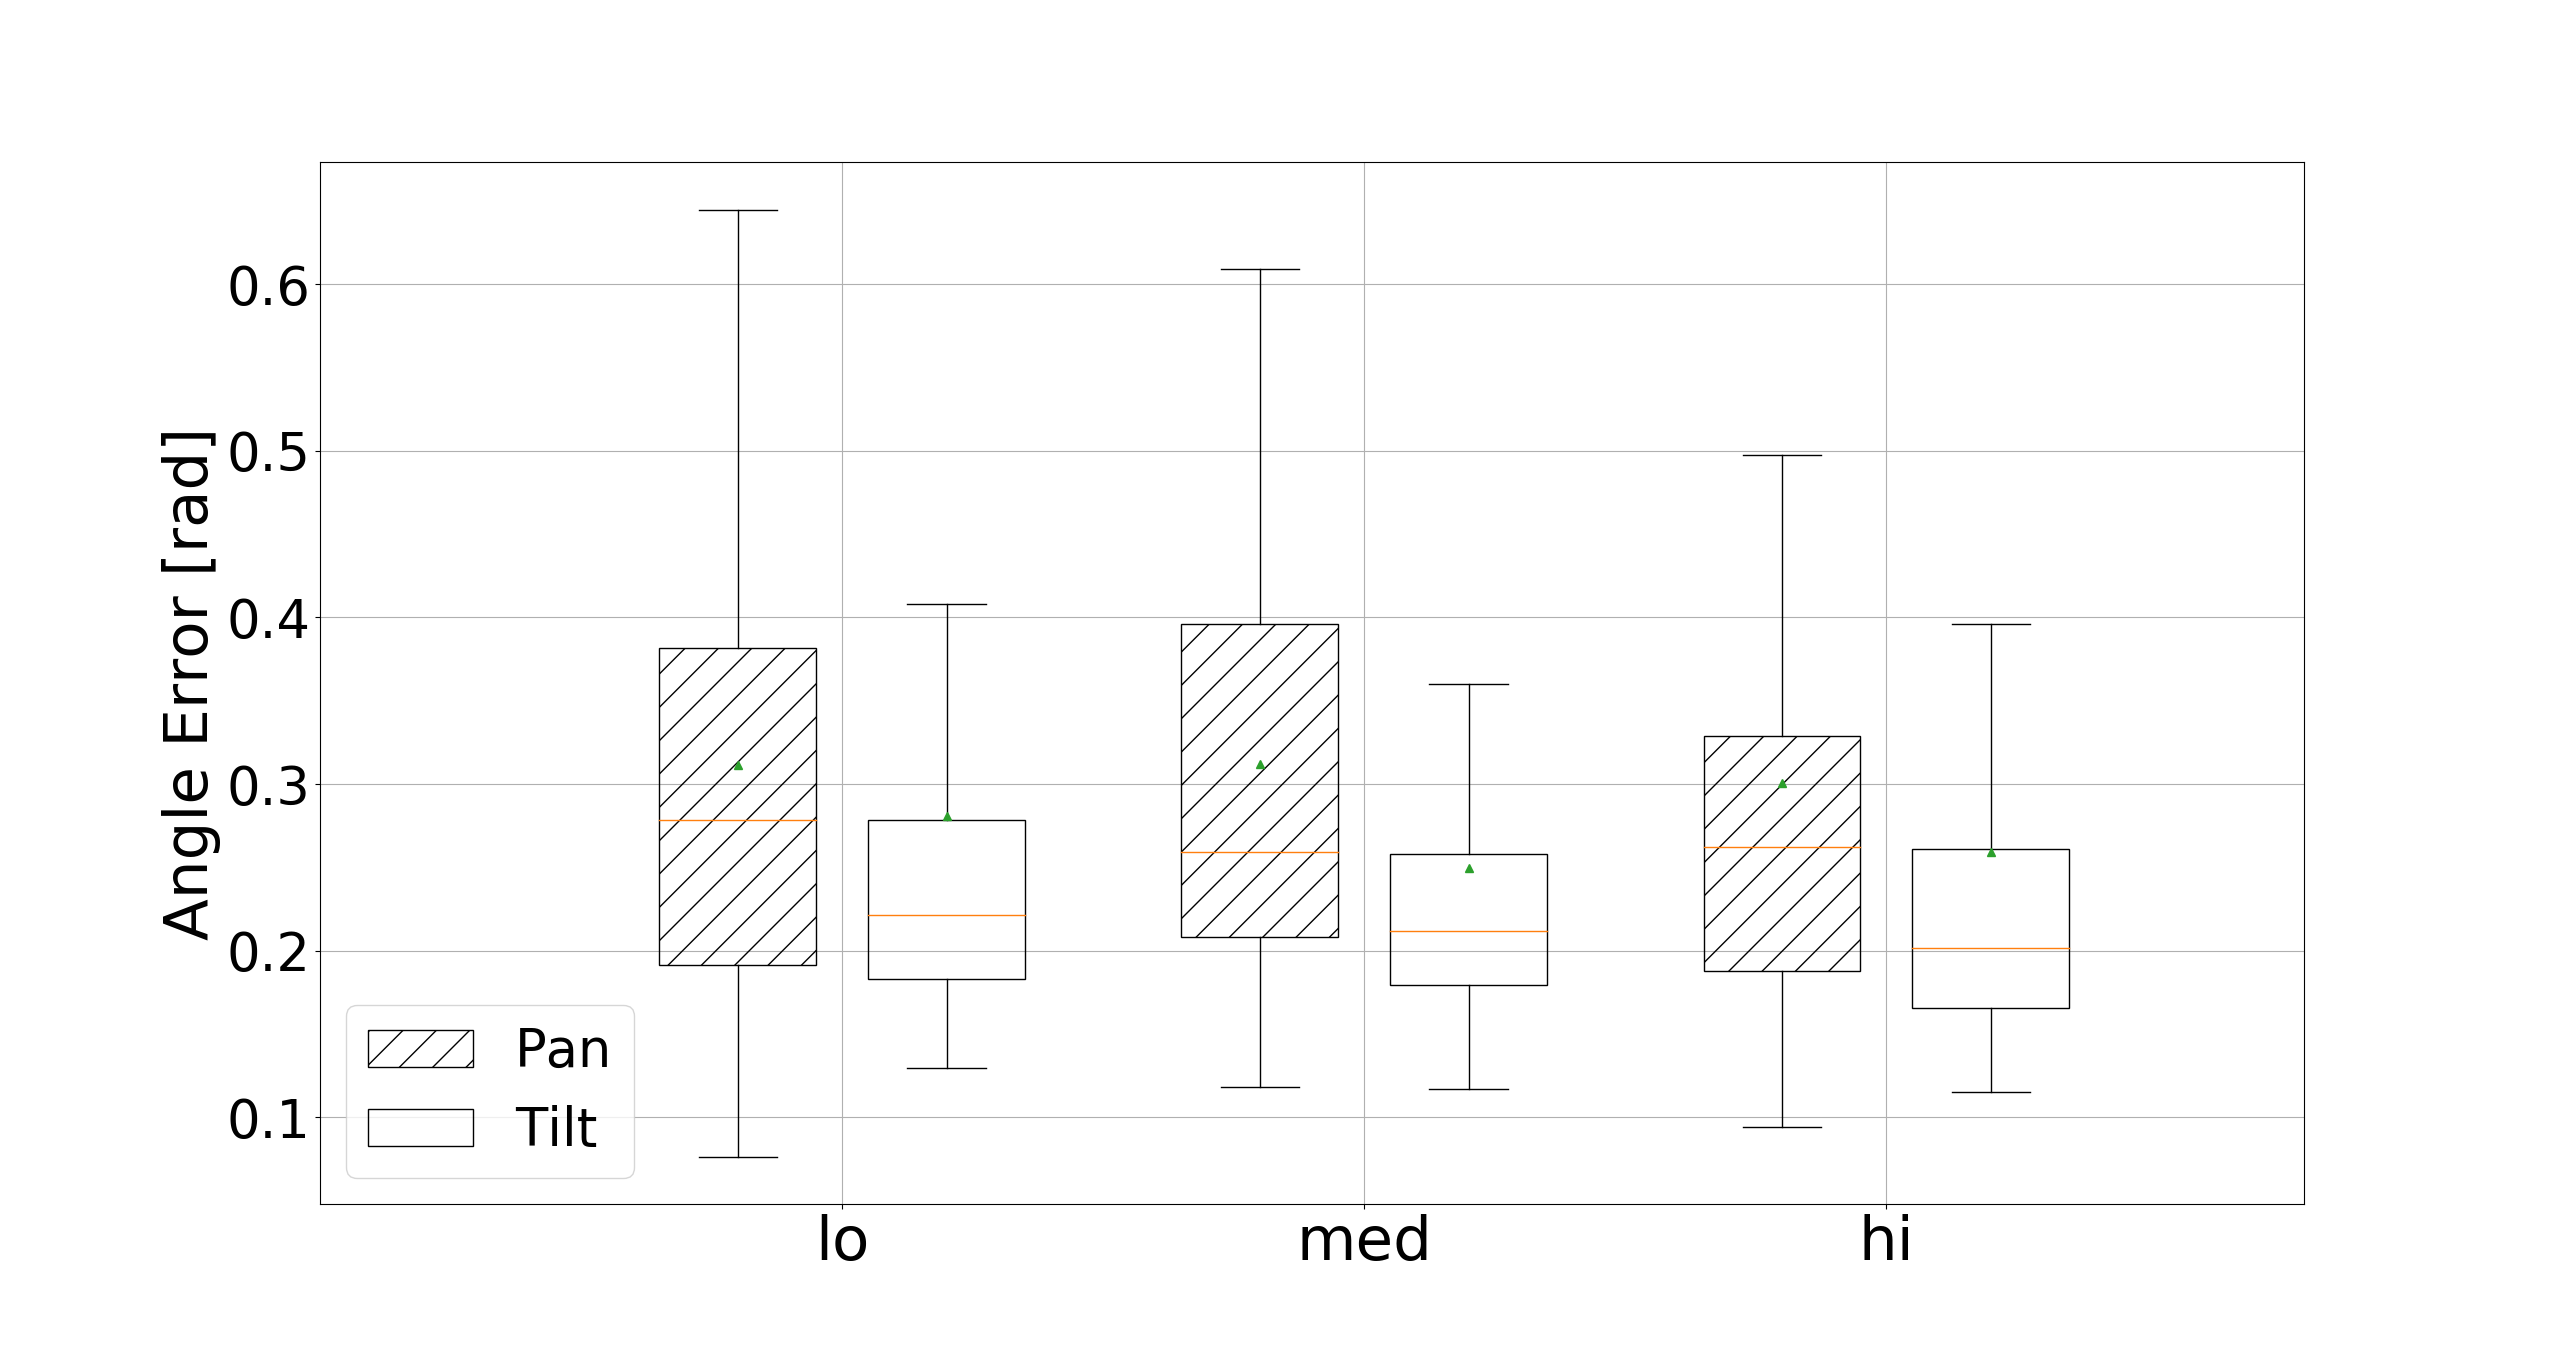
\includegraphics[clip, trim=80 -70 100 0, width=0.4\textwidth]{figures/err_boxplot_std.png}
  \caption{Error standard deviations.}
  \label{fig:err-boxplot-std}
\end{figure}

\begin{table}
  \centering
  \caption{A table of the pan and tilt angular error results for the target search experiment. The results include the absolute average error ($\mu_{abs}$), average error ($\mu$) and standard deviations ($\sigma$) given in radians, as well as the Spearman ($R$) correlation scores.}
  \label{tab:results}
  \begin{tabular}{|c|l|c|c|c|c|}
    \hline
    \multicolumn{2}{|c|}{} & $\mu_{abs}$ & $\mu$ & $\sigma$ & $R$ \\\hline\hline
    & \emph{lo}  & 0.23 & -0.02 & 0.32 & 0.75 \\\cline{2-6}
    Pan & \emph{med} & 0.21 & -0.01 & 0.28 & 0.77 \\\cline{2-6}
    & \emph{hi}  & 0.22 & -0.05 & 0.31 & 0.75 \\\hline\hline
    & \emph{lo}  & 0.40 & -0.14 & 0.46 & 0.38 \\\cline{2-6}
    Tilt & \emph{med} & 0.32 & -0.12 & 0.36 & 0.48 \\\cline{2-6}
    & \emph{hi}  & 0.34 & -0.16 & 0.39 & 0.55 \\\hline
  \end{tabular}
\end{table}

\crefrange{fig:err-results-lo}{fig:err-results-hi} and the median and mean points from the box-plots in \crefrange{fig:err-boxplot-median}{fig:err-boxplot-std} show that the data in the pan dimension is approximately normally distributed around zero.
However, $p$-scores below the critical 0.05 level from the Shapiro-Wilkes test and inspection of the quantile-quantile (Q-Q) plots do not give enough confidence to consider the data as normally distributed and we therefore analyse the data through non-parametric techniques. 

There is a strong linear correlation between the participants' guesses and the targets' true pan angles, shown by the high Spearman correlation scores of approximately 0.75 ($p \ll 0.05$) for all of the datasets, with the \emph{med} configuration displaying the marginally best result of 0.77.
The three settings have similar average errors and standard deviations, with the \emph{med} configuration again producing the marginally best results with the smallest average error and standard deviation.
However, the differences are small (approximately 6\%) and are not significant enough (Friedman test $p \gg 0.05$) to conclude that the pitch gradient has an effect on the performance in the pan dimension. 

The data collected from the participants with partial eyesight follow a similar trend to that of the blindfolded participants: the error in the pan dimension is centred around \SI{0}{\radian} with similar standard deviations across all three settings.
These results are summarised in Table~\ref{tab:vi-results}.
Unfortunately, not enough samples could be collected to draw any final conclusions.
However, these results are in line with results from previous work~\cite{zwiers2001spatial}, indicating that the groups with partial and normal eyesight respond with similar levels of accuracy to spatialised sound when presented with simple tasks. 

\begin{table}
  \centering
  \caption{A table summarising the target search results of the participants with partial eyesight (P1 - P3). The results include the average error ($\mu$) and standard deviation ($\sigma$), given in radians in the pan and tilt dimensions.}
  \label{tab:vi-results}
  \begin{tabular}{|c|c|cc|cc|cc|}
    \hline
    \multicolumn{2}{|c|}{} & \multicolumn{2}{c|}{\emph{lo}} & \multicolumn{2}{c|}{\emph{med}} & \multicolumn{2}{c|}{\emph{hi}} \\
    \multicolumn{2}{|c|}{} & $\mu_l$ & $\sigma_l$ & $\mu_m$ & $\sigma_m$ & $\mu_h$ & $\sigma_h$ \\\hline\hline
    & P1 & 0.25 & 0.44 & 0.21 & 0.45 & 0.29 & 0.40 \\ \cline{2-8}
    Pan & P2 & 0.18 & 0.85 & 0.05 & 0.49 & -0.08 & 0.32 \\ \cline{2-8}
    & P3 & -0.10 & 0.67 & -0.08 & 0.61 & -0.08 & 0.50 \\ \hline\hline
    & P1 & -0.17 & 0.21 & -0.10 & 0.2 & -0.25 & 0.21 \\ \cline{2-8}
    Tilt & P2 & -0.87 & 0.26 & -0.05 & 0.21 & -0.15 & 0.18 \\ \cline{2-8}
    & P3 & -0.57 & 0.31 & -0.57 & 0.45 & -0.38 & 0.39 \\ \hline
  \end{tabular}
\end{table}

Based on previous research~\cite{zwiers2001spatial}, these results were somewhat expected.
In addition, they also confirm that a participant's target search capability in the pan dimension is robust to the changing pitch for the target's tilt angle which is a useful result in support of the effectiveness of our audio interface.

\subsection{Tilt Results}\label{sec:tilt-results}

Besides the pan, the ordinates in \crefrange{fig:err-results-lo}{fig:err-results-hi} also show the results recorded during the target search experiment for the tilt direction.
A set of box-plots are given in \cref{fig:err-boxplot-median} to show the average tilt error between the participants' guesses and the targets' true positions.
All of the results are summarised in Table~\ref{tab:results}. 
The data here are also considered not normally distributed following inspections of the Q-Q plots and Shapiro-Wilkes test results and are analysed accordingly.

We found that there is reasonably significant correlation between the participants' guesses and the actual locations of the targets, shown by moderate Spearman correlation scores of approximately 0.38 for \emph{lo}, 0.48 for \emph{med} and the \emph{hi} gradient giving the strongest R-scores of the three with a score of 0.55 ($p \ll 0.05$ for all 3 settings).
This indicates that the varying pitch is working as expected and the participants are generally interpreting the cues correctly. 

The average errors of the datasets are relatively close to one another, with the \emph{lo} gradient giving the largest absolute error and standard deviation at \SI{0.40}{\radian} and \SI{0.46}{\radian}.
The \emph{med} and \emph{hi} have similar absolute errors of \SI{0.32}{\radian} and \SI{0.34}{\radian} respectively.
This is in line with the correlation scores, with the \emph{lo} gradient giving a worse result than the \emph{med} and \emph{hi} gradients and the \emph{hi} gradient giving the best results overall, with its high correlation score and relatively low absolute angular errors and standard deviation. 

We use the Friedman test~\cite{friedman1937use} on the medians of the data to find the statistical significance of the differences between the datasets.
We use the median values here since the data are not normally spread and there is significant noise within the data which may contaminate the mean values.
This results in a $p$-value of 0.002, which falls below the commonly-used critical threshold of 0.05, implying that there is a statistically significant difference between the three settings.
A post-hoc analysis with a Wilcoxon signed rank test and a critical threshold with a Bonferroni correction applied for the 3 settings ($\alpha=0.016$) shows that both the \emph{med} and \emph{hi} settings are significantly different than the \emph{lo} setting ($p=0.0014$ for both settings), but that the \emph{med} and \emph{hi} settings do not produce significantly different results from one another ($p=0.42$).
This is supported by the earlier observations made on the average and standard deviations of the error data which indicate that the \emph{lo} setting gives the highest average errors, while the \emph{med} and \emph{hi} settings produce similar error levels. 

From \cref{fig:err-boxplot-median} it can also be seen that the data show a significant skewing to the negative side, indicating a potential bias amongst the experiment's participant-base that must be taken into account.
From the results, it is not completely clear what causes this negative bias in the pitch dimension.
However, a possible explanation is that the floor introduces a position constraint within the participants' minds, since the target cannot appear below the ground.
It can potentially appear above the participants' head though, giving variable upper an lower limits that depend on the participants' height and individual perception.
Future improvements to our audio interface should consider a non-linear increase in pitch as a function of tilt angle instead of the linear one we used in this work to remedy this bias.
%\cref{fig:tone-threshold} shows the distribution of the cut-off frequency thresholds that were found in Section~\ref{sec:character}, as well as a plot of the median values of the errors in the tilt dimension, transformed to a frequency using each dataset's respective pitch-gain gradient. 

%In particular, \cref{fig:tone-medians} indicates that the participants, on average, searched for the target until they could no longer detect a difference between the tone they were played and the \SI{512}{\hertz} on-target tone they were searching for.
%This is shown by the vast majority of the error data being located below the 75\% cut-off threshold frequency of \SI{12.9}{\hertz} (0.43 semitones around \SI{512}{\hertz}).
%Furthermore, it can be seen that the \emph{hi} dataset comes the closest to the cut-off frequency.
%This could explain why it produces the strongest correlation between the targets' true perceived position, since the \emph{hi} pitch gradient is the most sensitive to changes in the tilt angle, it allowed the participants to get closer to the true tilt by playing a more easily distinguishable tone.

Given the small sample size, there is limited meaningful statistical analysis we can do on the data collected from the participants with visual impairments.
However, it could be seen from the results in Table~\ref{tab:vi-results} that these participants displayed the same behaviour in our experiments, with a clear bias toward the lower angles (i.e.\ the floor) and not-insignificant variability between the three settings in the tilt dimension.
Similarly, the pan dimension remains more stable throughout the three settings.
The participants also confirmed that they preferred the \emph{hi} setting, since it was more responsive and gave them a clearer idea of the direction they needed to point to. 

These results show that a varying pitch tone can convey the tilt angle of a target to a human using bone-conducting headphones with accuracy levels similar to that in the literature~\cite{bujacz2011sonification, katz2011spatial, zotkin2004rendering}. They also highlight a clear and significant difference between the three different pitch gain gradients, with the \emph{hi} pitch-gain marginally outperforming the \emph{med} gain setting and producing the results closest to the true tilt. 

\subsection{Time to Target}

\crefrange{fig:fitts-lo}{fig:fitts-hi} shows the box-plots of the target-search time as a function of the \emph{ID} of the targets.
Here, the bin interval is the smallest effective width, calculated from Equation~\ref{eq:fitts-performance}, between the three gradient settings.
We used the relation from Equation~\ref{eq:fitts-base} and fitted a logarithmic regression line for each participant.
The medians of the $a$ and $b$ parameters, from Equation~\ref{eq:fitts-base}, for all the subjects' regressions were used to plot the resulting lines of best fit, shown in \crefrange{fig:fitts-lo}{fig:fitts-hi}. 

\begin{figure}
  \centering
  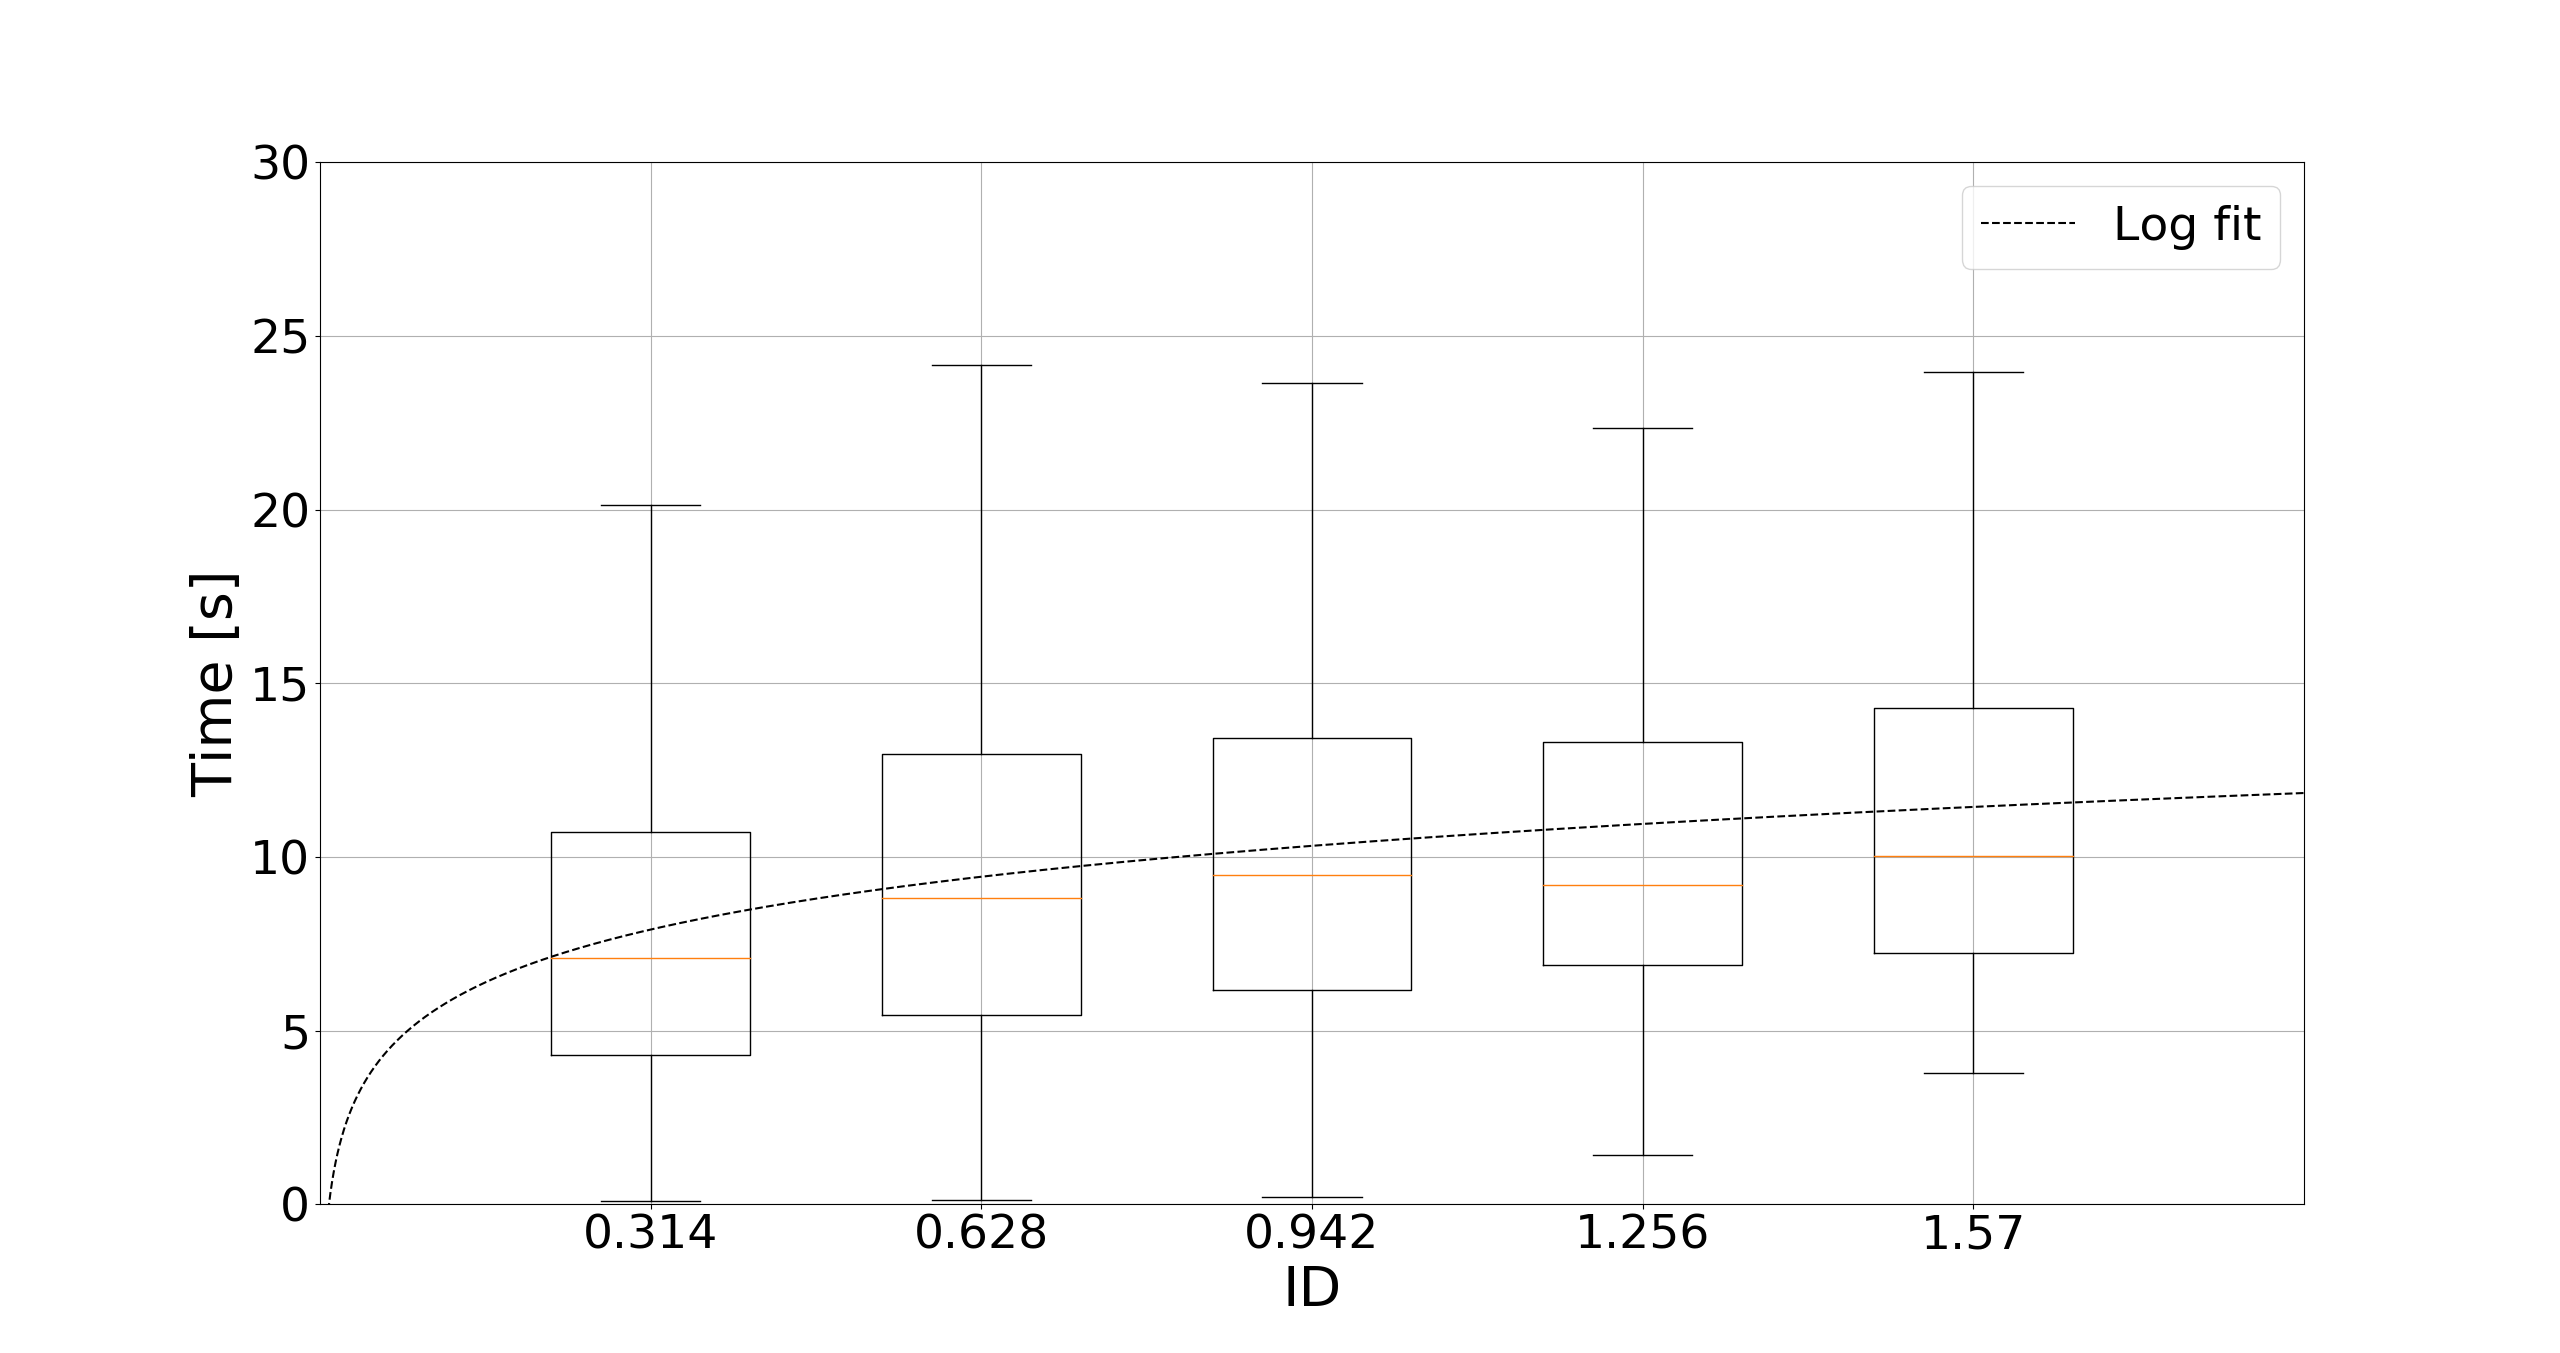
\includegraphics[clip, trim=120 20 120 20, width=0.4\textwidth]{figures/fitts_lo.png}
  \caption{\emph{Lo} setting. }\label{fig:fitts-lo}
\end{figure}

\begin{figure}
  \centering
  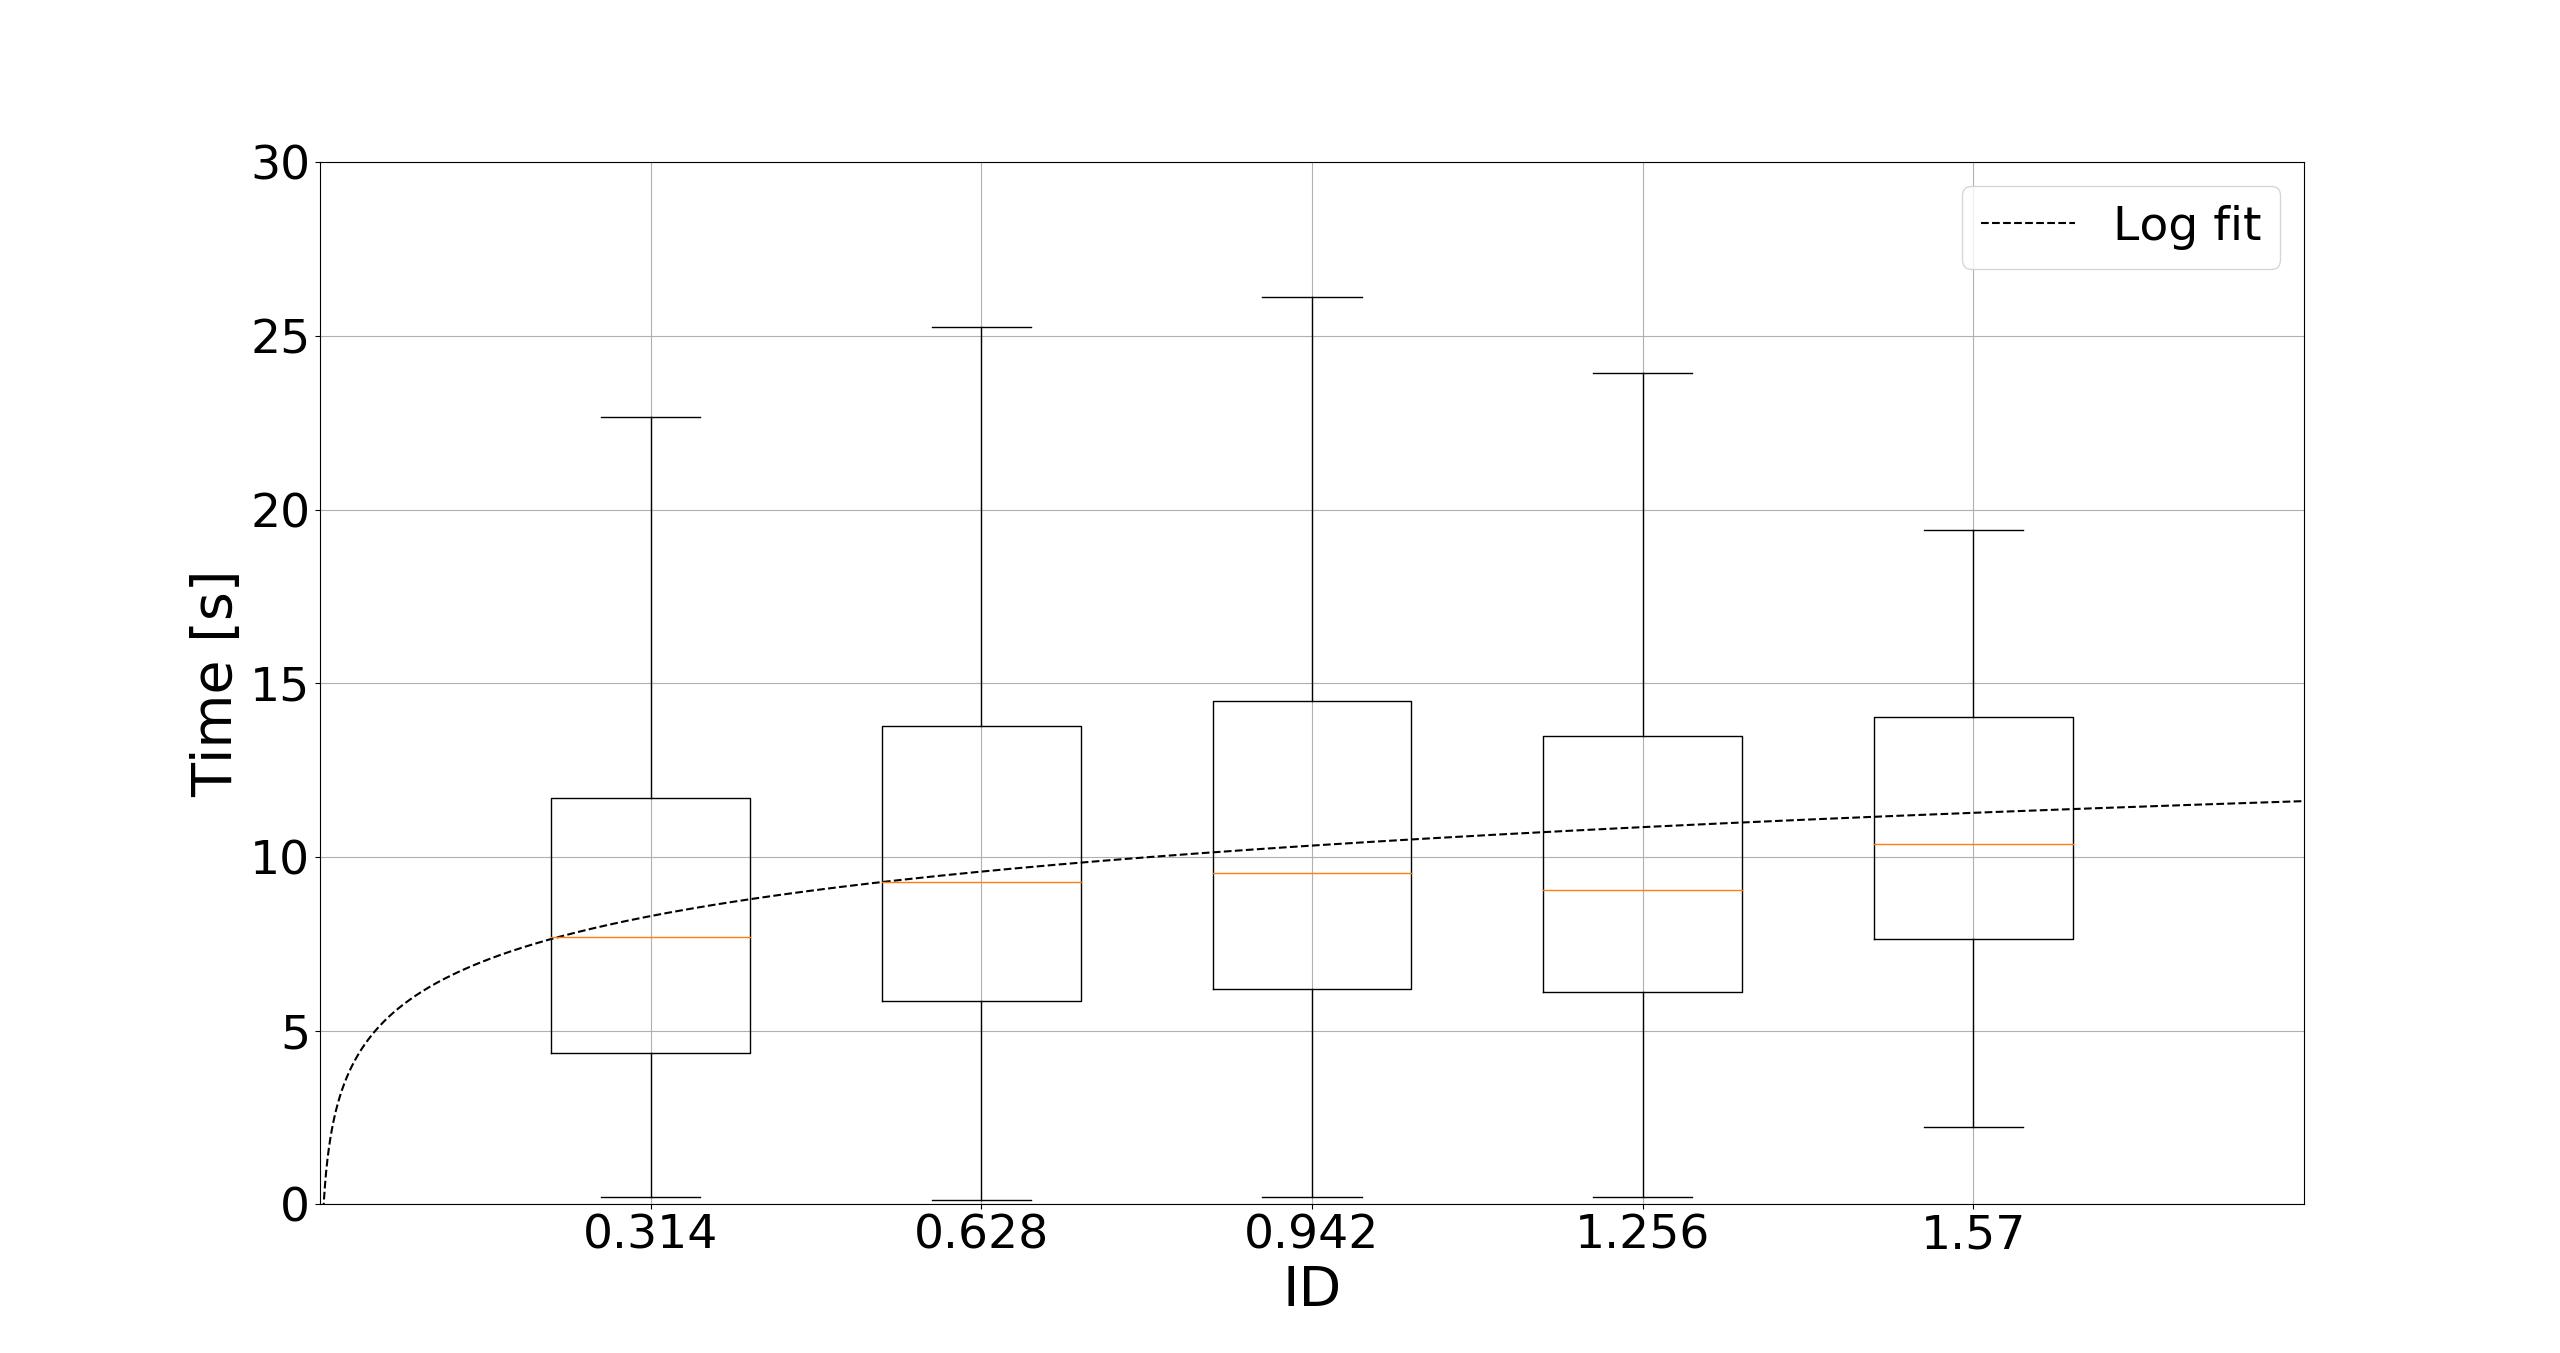
\includegraphics[clip, trim=120 20 120 20, width=0.4\textwidth]{figures/fitts_med.png}
  \caption{\emph{Med} setting. }
  \label{fig:fitts-med}
\end{figure}

\begin{figure}
  \centering
  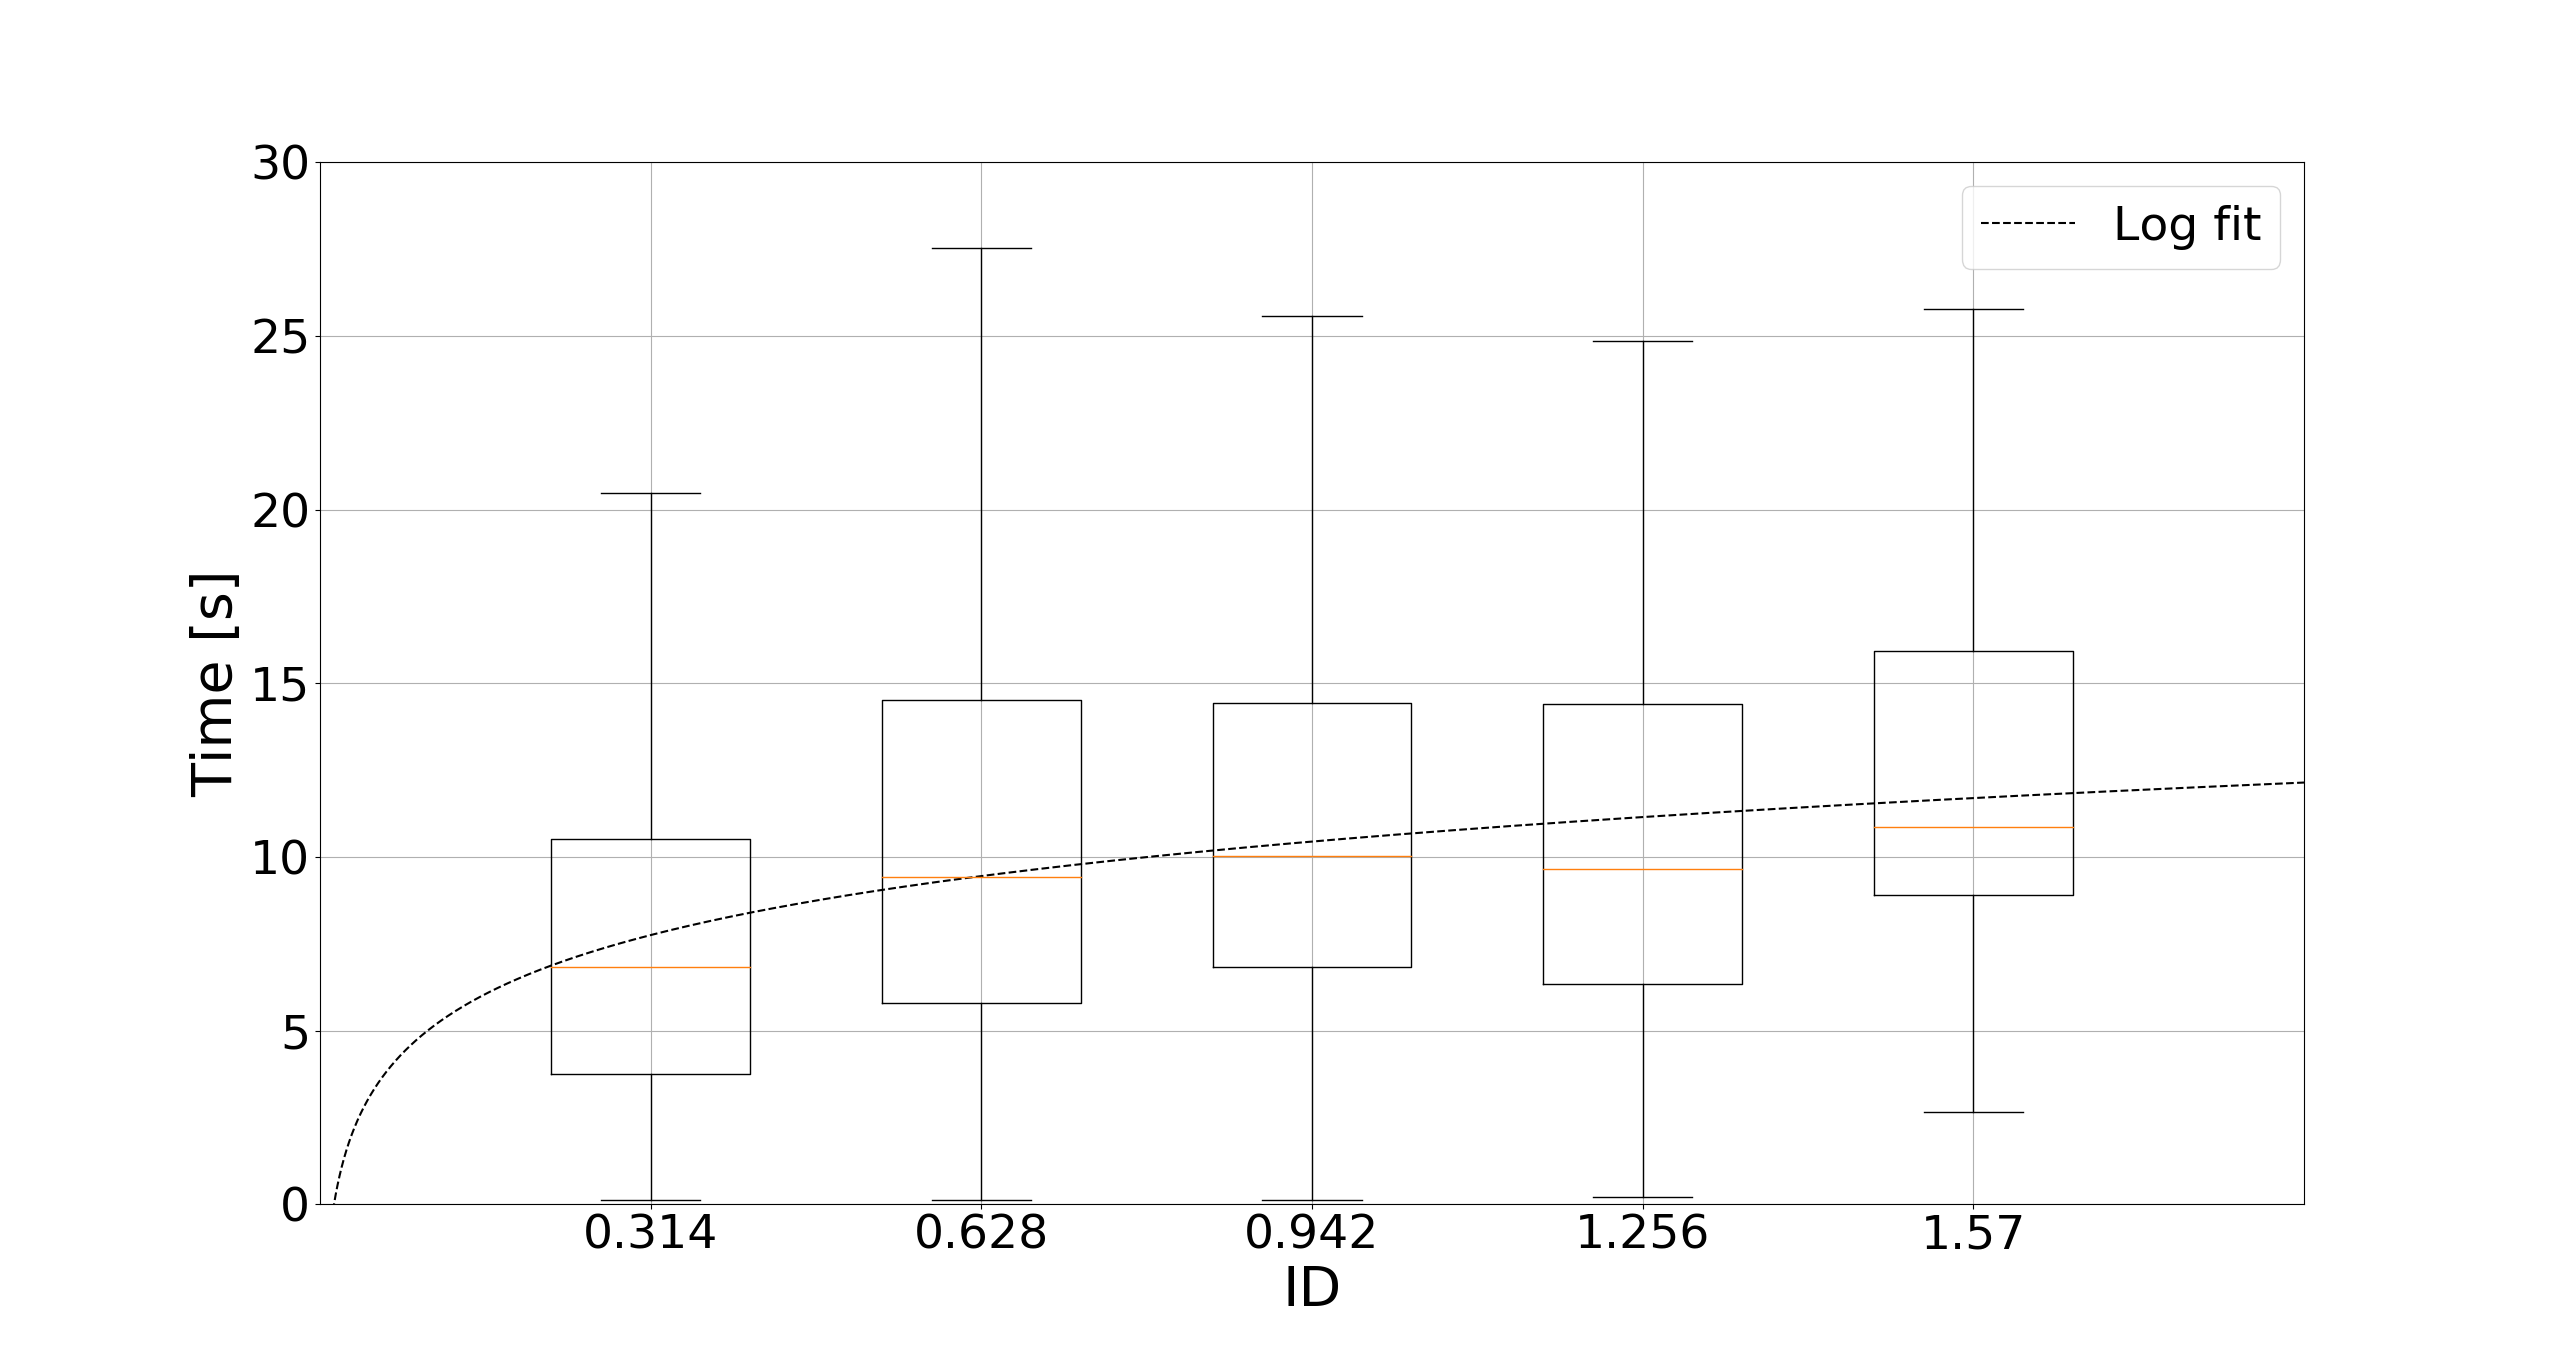
\includegraphics[clip, trim=120 20 120 20, width=0.4\textwidth]{figures/fitts_hi.png}
  \caption{\emph{Hi} setting. }
  \label{fig:fitts-hi}
\end{figure}

\begin{figure}
  \centering
  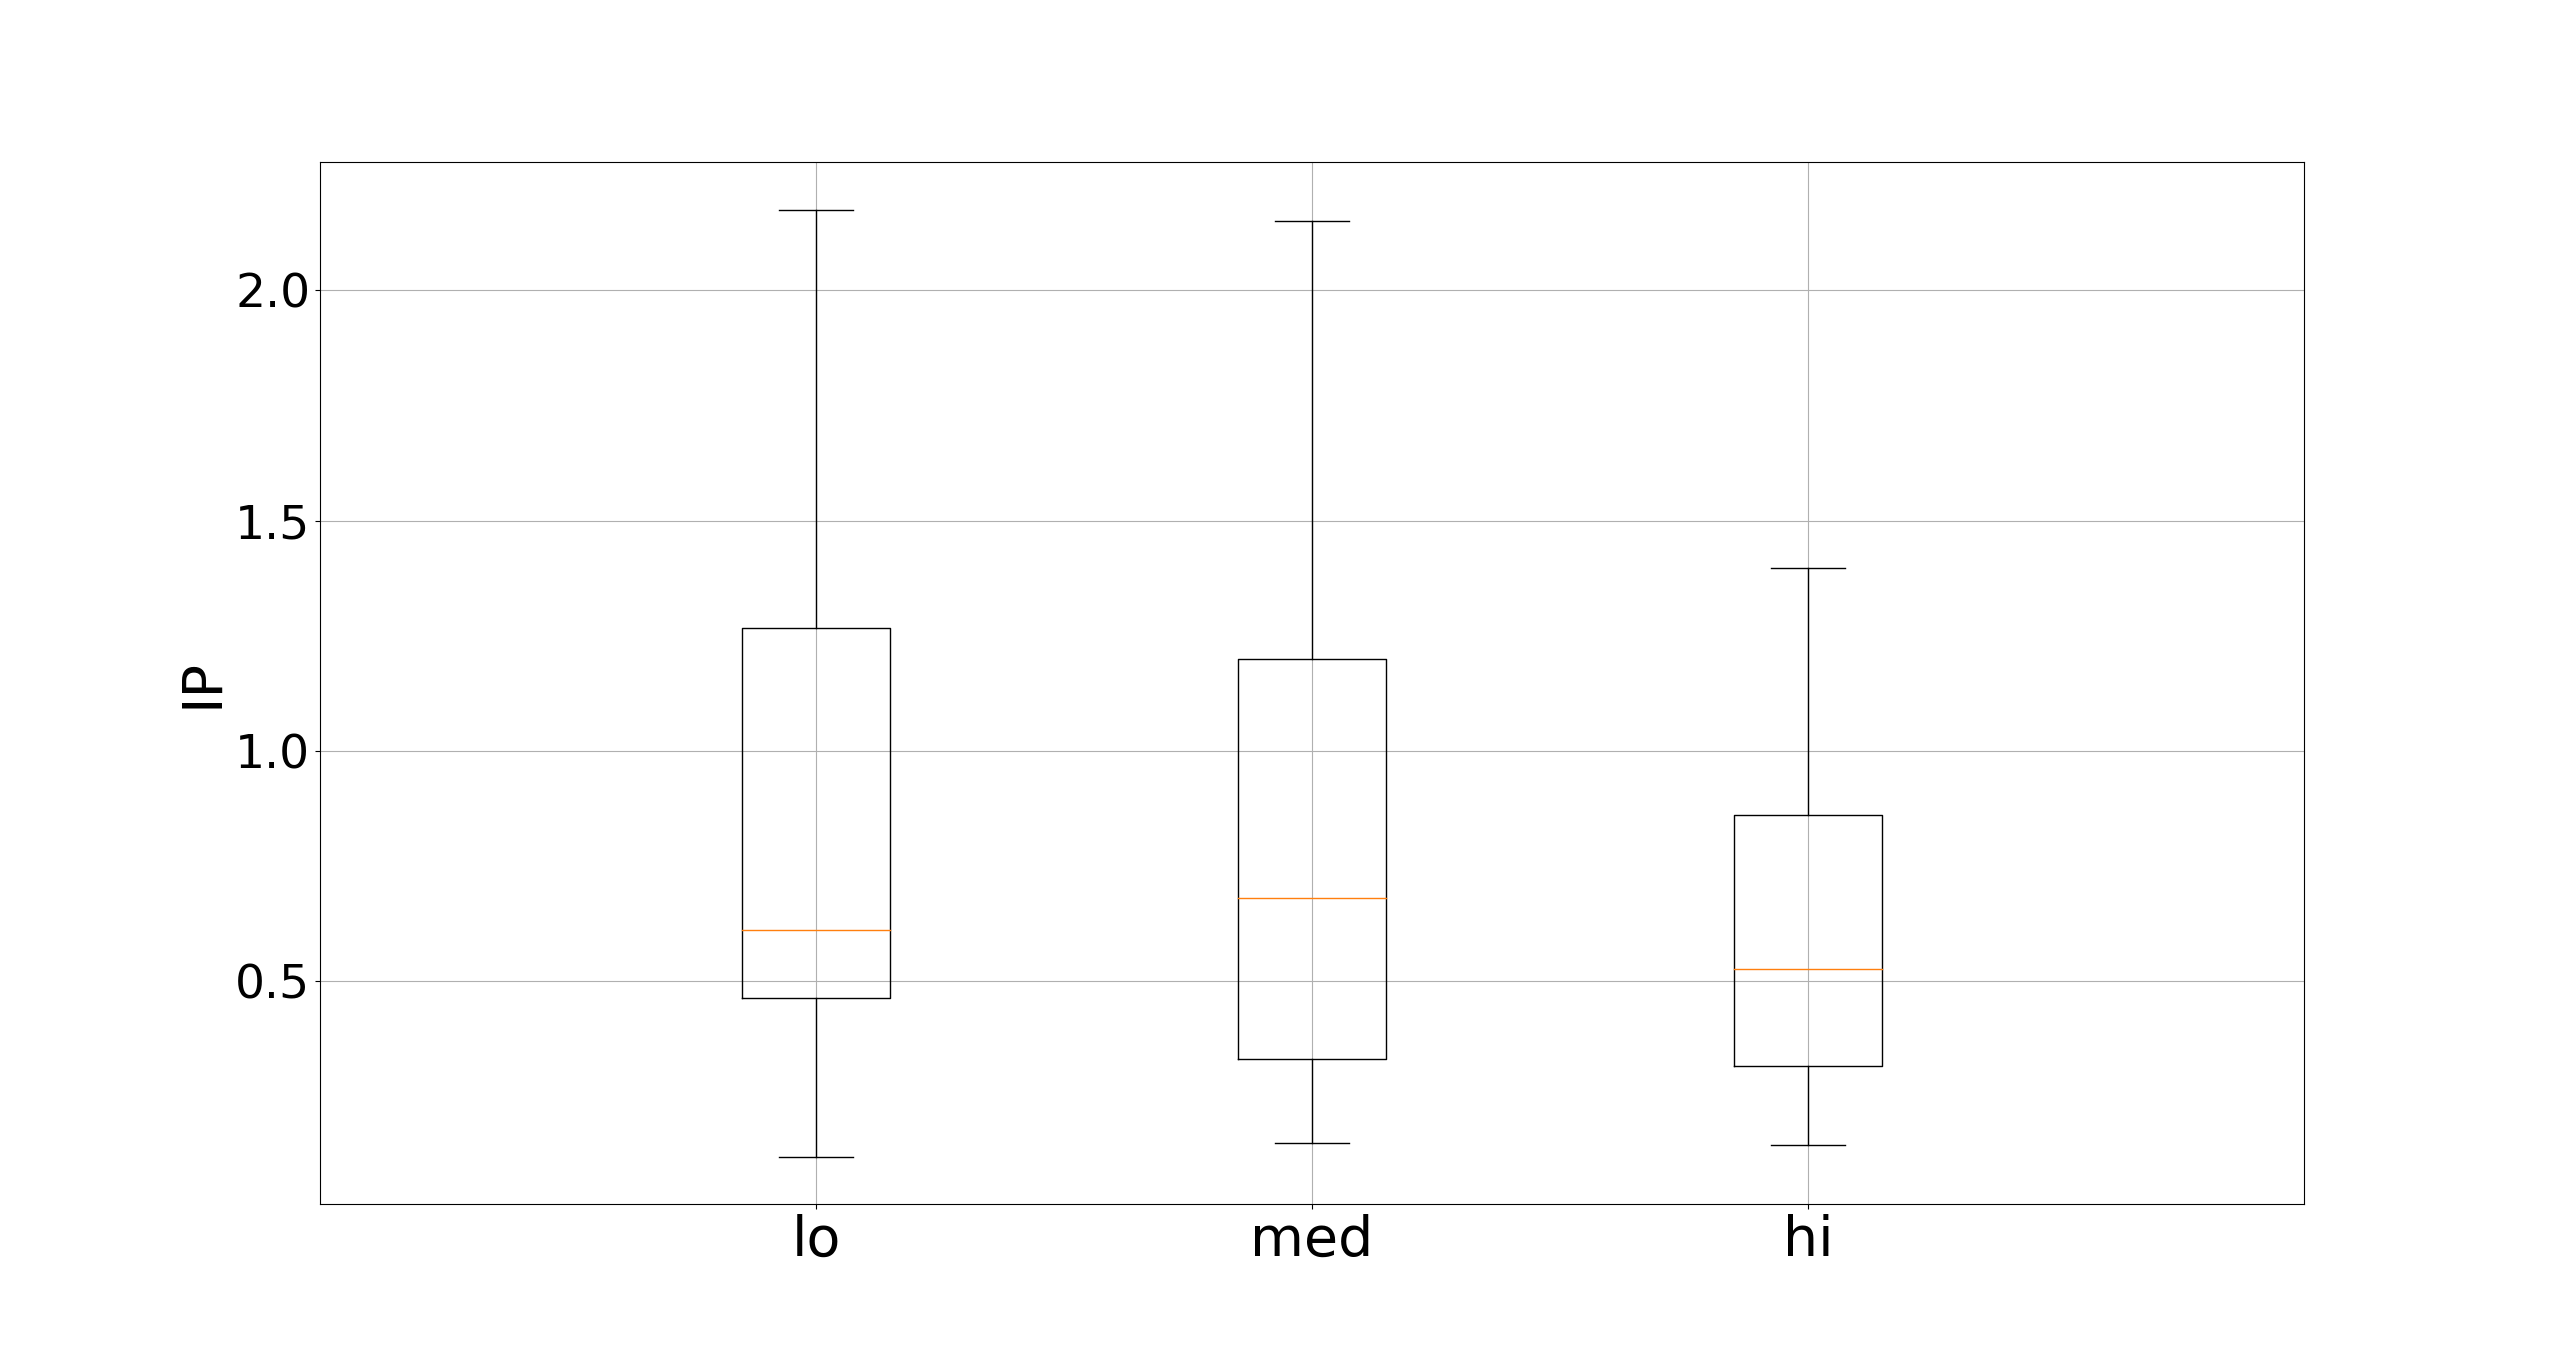
\includegraphics[clip, trim=90 20 130 20, width=0.4\textwidth]{figures/fitts_performance.png}
  \caption{Boxplots of the indices of performance.}
  \label{fig:fitts-performance}
\end{figure}

From these figures we can see that the data are consistent with Fitts's Law where the logarithmic line of best fit very closely approximates the median values of the binned data for all three pitch gradient settings, with each settings giving Pearson scores of 0.95, 0.87 and 0.93 for the \emph{lo}, \emph{med} and \emph{hi} settings respectively ($p < 0.05$ for all settings). 
This result enabled us to compute the index of performance, $IP$, given by Equation~\ref{eq:fitts-performance}, for all of the subjects.
These results were used to plot \cref{fig:fitts-performance}, which shows that the \emph{lo} and \emph{med} configurations give similar results, but slightly different spreads, while the \emph{hi} gives a lower $IP$.
The Friedman score for the three settings gives a $p$-value of 0.017, comfortably achieving statistical significance with a threshold of $\alpha=0.05$.
The Wilcoxon test comparing the \emph{lo} and \emph{hi} settings achieves significance after applying a Bonferroni correction ($\alpha=0.016$), but the other comparisons do not achieve significance. 

A possible explanation for the observed behaviour is that the more distinguishable changes in the audio pitch with the \emph{hi} configuration better informs the user when they are on target, leading to a more accurate estimate, but also increases the time it takes to point in the right direction.
Conversely, the \emph{lo} and \emph{med} gradients make it more difficult for the user to know when they are on target, leading to a shorter search time, but at the cost of lower accuracy.
This is confirmed by the results obtained in Section~\ref{sec:tilt-results} and the Wilcoxon test results. 

The results collected from the participants with partial eyesight follow the same trends observed in the blindfolded participants, giving $IPs$ of 0.58, 1.3 and 0.35 for the \emph{lo}, \emph{med} and \emph{hi} gradient settings respectively.  

\subsection{Participant with Visual Impairments' Feedback}

After and during the experiments involving the participants with visual impairments, we had the opportunity to collect their feedback on the current system implementation and suggestions for future improvements.

In general, they were satisfied with the current implementation and had little difficulty using it.
Furthermore, the prohibitive cost, complexity and cumbersomeness of other existing systems discouraged our subjects from purchasing and using them, so they were quite enthusiastic about our goal of developing a mobile or tablet-based indoor navigation system. 

One aspect of the audio interface that requires improvement is the tone used during the experiments was not very pleasant and led to auditory fatigue after a long period of use.
We are aware of this issue and we are already investigating more natural, `pleasant' and rich sounds to replace the basic sinusoidal wave that was used in the experiments.
One possibility is to use musical instruments (e.g.\ MIDI sound files) to play notes and scales~\cite{brewster1998using}.

Concerning the bone-conducting headsets, only one participant had reservations about this choice, citing cost concerns.
None of the participants had any technical issues in using the headset or misunderstanding audio cues.
They all agreed that this is a valid choice to avoid cutting a person with visual impairments off from environmental sounds.
Furthermore, they suggested to add some voice component to the system to inform the user of important events (e.g. \emph{`Target has been found'}, \emph{`You are veering off course'}, etc.) or to simply confirm and reassure the user that they are still on course.

%The final major suggestion was to add some form of on-target confirmation, either voice, vibration or some other audio cue. For the purposes of this experiment, we purposefully opted to not inform the participant when they were on target, since we are interested in the target acquisition accuracy. However, going forward we intend on adding an on-target notification in the form of an additional tone overlaid over the main tone. 

\section{Conclusion and Future Work}\label{sec:conclusion}

In this paper, we presented a spatial audio interface to direct a user with visual impairments to point a camera toward a target. We also discussed a set of experiments to determine its effectiveness and performance, as well as some subjective feedback collected from participants with partial eyesight. 

We found that a spatial audio tone with a varying pitch can be used to convey the pan and tilt angles of a target using a set of bone-conducting headphones.
The angular errors made by the participants are in line with those found in previous studies using similar audio interfaces.
We also found that varying the pitch-gain gradient of our interface influences the accuracy of the system in the tilt dimension, as well as the time to target, without affecting the performance in the pan dimension.
The steeper, \emph{hi}, pitch-gain was found to produce the best results in this respect.
Furthermore, we discovered a logarithmic relationship between the index of difficulty of a target and the time taken by a participant to find it, confirming that the results with our interface adhere to Fitts's Law.
However, there is a compromise to be made between speed and accuracy, with the \emph{hi} pitch-gain gradient directing the user to the target in the longest time. 

Feedback from the participants with visual impairments was mostly positive and they agreed with the choice of bone-conduction headphones that do not inhibit normal hearing.
However, they noted that the sine wave audio signal induced some audio fatigue, something noted by the other participants as well, and suggested suggested that more full-bodied, natural sounds be used instead.
Using vocal feedback in conjunction with the current audio signal was also suggested. 

Future research will focus on integrating voice and vibration feedback cues into the system.
We are also investigating solutions to automatically refine the parameters of the HMI and better match the individual user's navigation habits and capability, thereby increasing navigation performance and user satisfaction.

\bibliographystyle{ACM-Reference-Format}
\bibliography{bib}

\end{document}
